\documentclass[12pt]{report}
\usepackage{amsmath}
\usepackage{amssymb}
\usepackage{multirow}
\usepackage{hhline}
\usepackage{graphicx}
\usepackage{tikz}
\usepackage{longtable}
\usepackage{array}


\usetikzlibrary{tikzmark}

\newcommand{\linkV}[2]{%
	\begin{tikzpicture}[remember picture, overlay]
		\draw ([shift={(2mm, 6.6mm)}]{pic cs:#1}) to ([shift={(2mm, -2.8mm)}]{pic cs:#2});
	\end{tikzpicture}
}
\newcommand{\linkVV}[4]{%
	\begin{tikzpicture}[remember picture, overlay]
		\draw ([shift={(#3mm, 6.6mm)}]{pic cs:#1}) to ([shift={(#4mm, -2.8mm)}]{pic cs:#2});
	\end{tikzpicture}
}
\newcommand{\linkH}[2]{%
	\begin{tikzpicture}[remember picture, overlay]
		\draw ([shift={(-2mm, 2mm)}]{pic cs:#1}) to ([shift={(10mm, 2mm)}]{pic cs:#2});
	\end{tikzpicture}
}

\newcommand{\bt}[1]{\textbf{#1}}
\newcommand{\ubt}[1]{\textbf{\underline{#1}}}
\newcommand{\sps}{\\[0.2cm]}
\newcommand{\spn}[1]{\\[#1cm]}
\newcommand{\refn}[1]{\textbf{(\ref{#1})}}
\newcommand{\NI}{\noindent}
\newcommand{\dsp}{\displaystyle}
%%%%%%%%%%%%%%%%TERMS%%%%%%%%%%%%%%
\newcommand{\tp}{Transportation Problem }
\newcommand{\stp}{transportation problem }
\newcommand{\stps}{transportation problems }
\newcommand{\uwe}{Unilorin Water Enterprise }
\newcommand{\uwee}{Unilorin Water Enterprise(UWE) }


\renewcommand*\contentsname{Table of Contents}
\renewcommand{\baselinestretch}{1.5}
\renewcommand{\arraystretch}{1.2}


\begin{document}
		%%remove the numbering from the first page 
	\clearpage
	\thispagestyle{empty}
	%%TITLE%%
	\addcontentsline{toc}{chapter}{TITLE PAGE}
	\begin{center}
		{\bf \LARGE TRANSPORTATION PROBLEM}\sps
		{\bf \Large A Case Study Of Unilorin Water Enterprise(UWE)}
	\end{center}
	$$$$
	\begin{center}
		\textbf{\itshape BY}
	\end{center} 
	$$$$
	\begin{center}
		{\bf David, Udo Uduak\\
			17/56EB094}
	\end{center}
	$$$$
	\begin{center}
		\textbf{A PROJECT SUBMITTED TO THE
			DEPARTMENT OF MATHEMATICS, FACULTY OF PHYSICAL SCIENCES,
			UNIVERSITY OF ILORIN, ILORIN, NIGERIA,
			$$$$
			IN PARTIAL 
			FULFILMENT OF REQUIREMENTS FOR THE AWARD OF
			BACHELOR OF SCIENCE (B.Sc.) DEGREE IN MATHEMATICS.}
	\end{center}
	$$ $$ 
	\\ \\
	\begin{center}
		{\bf NOVEMBER, 2022}
	\end{center}
	\newpage
	\pagenumbering{roman} 
	\addcontentsline{toc}{chapter}{CERTIFICATION}
	\section*{\begin{center}\textbf{\Large CERTIFICATION}   \end{center}}
	This is to certify that this project work was carried out by \textbf{David, Udo Uduak} with matriculation number \textbf{17/56EB094} and approved as meeting the requirement for the award of the Bachelor of Science (B. Sc.) degree of the Department of Mathematics, Faculty of Physical Sciences, University of Ilorin, Ilorin, Nigeria.
	\\
	\\
	................................... \qquad \qquad\qquad\qquad\qquad\qquad...................... \\
	Prof. M.O. Ibrahim  \quad\qquad\qquad\qquad\qquad\qquad\qquad\qquad Date\\
	Supervisor\\
	\\
	\\
	\\
	...................................... \qquad\qquad\qquad\qquad\qquad\qquad ......................\\
	Prof. K. Rauf      \qquad\qquad\qquad\qquad\qquad\qquad\qquad\qquad\quad     Date\\
	Head of Department\\
	\\
	\\
	\\
	..................................... \qquad\qquad\qquad\qquad\qquad\qquad .......................\\
	Prof.  \quad\qquad\qquad\qquad\qquad\qquad\qquad\qquad         Date\\
	External Examiner
	
	\newpage
	%%DEDICATION%%
	\section*{\begin{center}\textbf{\Large DEDICATION}\end{center}}
	\addcontentsline{toc}{chapter}{DEDICATION}
	This is dedicated to God Almighty, my creator, my strong pillar, my source of inspiration, wisdom, knowledge, and comprehension. He has been the source of my strength throughout this program, and I have soared only on his wings.\\
	
	\NI I also dedicate this work to my father, Apostle David Udosen, who has always encouraged me and ensured that I give it everything I have to finish what I started. Aduragbemi Olorunyomi; my buddy turned sister, thank you for everything you do for me. And to my friends, course-mate, family, and well-wishers; my love for you all is immeasurable. God's blessings on you all.

	
	\newpage
	%%ACKNOLEDGMENTS%%
	\section*{\begin{center}\textbf{\Large ACKNOWLEDGMENTS}\end{center}}
	\addcontentsline{toc}{chapter}{ACKNOWLEDGMENTS} 					
	All praises, adoration and glorification are for Almighty God.\\
	
	\NI My profound gratitude and appreciation go to my protean and persisting supervisor, Prof. M. O. Ibrahim, for his kind- heartedness, and for his candid advice, encouragement and useful guidelines towards the success of this project. I pray that the Almighty God be with him and his family.\\
	
	\NI I acknowledge my level adviser Dr. K. A. Bello for his support and help when required, I’m really grateful.\\
	
	\NI I also extend my sincere gratitude to the Head of Department, Prof. K. Rauf and also to all my esteem Lecturers: Prof. J. A. Gbadeyan, Prof. T. O. Opoola, Prof. O. M. Bamigbola, Prof. O. A. Taiwo, Prof. M. O. Ibrahim, Prof. R. B. Adeniyi, Prof. S. O. Makanjuola, Prof. M. S. Dada, Prof. A. S. Idowu, Prof. E. O. Titiloye,  Prof. O. A. Fadipe-Joseph,  Dr. Yidiat O. Aderinto, Dr. Catherine N. Ejieji, Dr. B. M. Yisa, Dr J. U. Abubakar, Dr. Gata N. Bakare, Dr T. O. Olotu, Dr. B. M. Ahmed, Dr Idayat F. Usamot, Dr O. A. Uwaheren, O. Odetunde and all other members of staff of the department of mathematics, who contributed greatly to my academic excellence, obtained during my period of study in the department. May God bless them all.\\
	
	\NI I also want to thank the Manager of Unilorin Water Enterprise (UWE) for providing the data for the study.
	
	
	\newpage
	%%ABSTRACT%%
	\section*{\begin{center}\textbf{\Large ABSTRACT}\end{center}}
	\addcontentsline{toc}{chapter}{ABSTRACT}
	This study takes into account the proposed transportation model of manufacturing goods to consumers (key distributors).\\
	
	\NI This transportation model will be useful for Unilorin Water Enterprise logistics managers in making strategic decisions regarding the optimal allocation of products from four storehouses; factory, consultancy, business school, and UITH, to various customers (key distributors) at the lowest transportation cost.
	
	%%TABLE OF CONTENTS%%
	\addcontentsline{toc}{chapter}{TABLE OF CONTENTS}
	\tableofcontents
	\newpage
	
	\pagenumbering{arabic}
	%%%%%%%%%%%%%%%%%%%%%%%%%CHAPTER ONE%%%%%%%%%%%%%%%%%%%%%%%%%%%%
	\chapter{GENERAL INTRODUCTION}
	
	\section{Introduction}
	The \bt{\tp (TP)} is the overall term for a wide range of issues in which transportation is required. The following are the general parameters of Transportation Problem:
	\begin{enumerate}
		\renewcommand{\labelenumi}{(\Alph{enumi})}
		\item \bt{Resources:} These are the elements that can be moved from one location to another. Goods, machinery, tools, people, and cargo are examples of discrete resources; continuous resources include energy, liquids, and money..
		
		\item \bt{Locations:} Point of delivery, recollection depots, nodes, railway stations, bus terminals, loading ports, seaports, airports, refueling depots, and schools are all examples of locations.
		
		\item \bt{Transportation Modes:} Transportation modes are methods of delivering resources to certain areas. Water, space, air, road, train, and cable are used as forms of transportation. The infrastructure, capacity, schedules, activities, and rules varies depending on the mode of transportation. Ships, planes, trucks, trains, pipelines, motorcycles, and other forms of movement are examples.
	\end{enumerate}
		\section{Types of Transportation Problem}
	There are basically two (2) types of transportation problem:
	\begin{enumerate}
		\item Balanced \tp\\[-1.1cm]
		\item Unbalanced \tp \\[-1.3cm]
	\end{enumerate}
	\begin{figure}[!h]
		\centering
		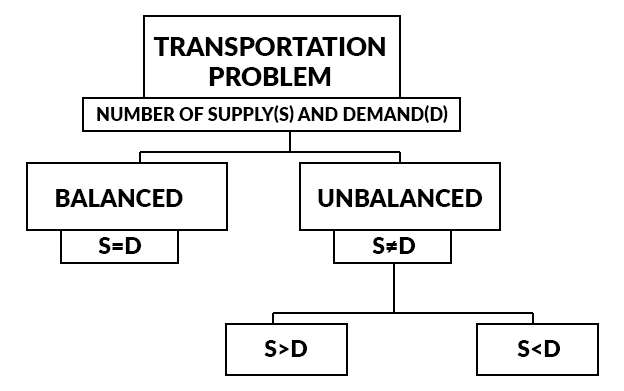
\includegraphics[width=0.51\linewidth]{tt4}
		\caption{Types of Transportation Problem}
		\label{fig:1_1}
	\end{figure}
	
		\section{Model of A \tp}
	The \stp model is defined by
	\begin{gather}
		\text{Minimize } Z = \sum_{i=1}^{m}X_{ij}C_{ij}\label{eq:3_1}\sps
		\sum_{j=1}^{n}X_{ij} \leq a_i~~,~~ i=1,2,3,\ldots,m~~ (\text{Demand Constraint}\label{eq:3_2}\sps
		\sum_{i=1}^{m}X_{ij} \geq b_j~~,~~ j=1,2,3,\ldots,n~~ (\text{Supply constraint})\label{eq:3_3}\sps
		X_{ij} \geq 0,1,2,3,\ldots,n\label{eq:3_4}
	\end{gather}
	
	\NI This is a Linear Program with $m\cdot n$ decision variables, $m+n$ functional constants, and $m\cdot n$ non-negative constraints. Where\sps
	$n$ is the number of destination\\
	$m$ is the number of resources\\
	$a_i$ is the capacity of $i$ source\\
	$b_j$ is the demand of $j$th destination\\
	$C_{ij}$ is the unit transportation cost between $i$th source and $j$th destination (in naira or as a distance in Kilometers, miles, etc.). While $X_{ij}$ is the size of material transported between $i$th source and $j$th destination (in tons, pounds, liters etc.).\sps
	
	\NI A \stp is said to be unbalanced if and only if
	\begin{eqnarray}
		\sum_{i=1}^{m}a_i \neq \sum_{j=1}^{n}b_j\label{eq:3_5}
	\end{eqnarray} 
	
	\NI There are two cases:\\
	Case (1)
	\begin{eqnarray}
		\sum_{i=1}^{m}a_i \geq \sum_{j=1}^{n}b_j\label{eq:3_6}
	\end{eqnarray}
	Case (2)
	\begin{eqnarray}
		\sum_{i=1}^{m}a_i \leq \sum_{j=1}^{n}b_j\label{eq:3_7}
	\end{eqnarray}
	
	\NI To balance the Transportation Problem, introduce a dummy origin or source in the transportation table with a zero cost. The availability at the origin is
	\begin{eqnarray}
		\sum_{i=1}^{m}a_i - \sum_{j=1}^{n}b_j = 0 \label{eq:3_8}
	\end{eqnarray}

%	\section{Mathematical Model of \tp}
%	In a typical \tp, a homogeneous product is to be transported from each of $m$ sources to any of $n$ destinations and their capacities are $a_1, a_2,\ldots,a_n$ and $b_1, b_2,\ldots, b_n$ respectively. In addition there is a penalty $c_{ij}$ associated with transporting a unit of the product from source $i$ to destination $j$. The penalty could represent transportation cost, delivery time, quantity of good delivered, safety delivery and many others. A variable $X_{ij}$ represents the unknown quantity to be transported from source $i$ to destination $j$. In the real life, all transportation problems are not single objective. Thus in general, the objective will also be controversial. In this paper, those \stps are considered, which are described by multiple objective functions.\\
%	
%	\NI The mathematical model of the multi-objective \stp is written as follows
%	\begin{eqnarray}
%		s_1: \text{Minimize } Z_k(x) = \sum_{i=1}^{m}\sum_{j=1}^{n}C_{ij}^k x_{ij}, \quad k=1,2,\ldots,k 
%	\end{eqnarray}
%	subject to
%	\begin{eqnarray*}
%		\sum_{i=1}^{m}x_{ij} &=& a_i \qquad\qquad i=1,2,\ldots,m\sps
%		\sum_{i=1}^{n} x_{ij} &=& b_j \qquad\qquad j=1,2,\ldots,n\\[-1.5cm]
%	\end{eqnarray*}
%	\begin{gather*}
%		x_{ij} \geq 0, \qquad \forall~~ i \text{ and } j
%	\end{gather*}
%	Where $\dsp Z_k(x) = \left\{Z_1(x), z_2(x),\ldots, Z_k(x)\right\}$ is a vector of $k$ objective functions, the subscripts on $Z_k(x)$ and superscript on $C^k_{ij}$ are used to identify the number of objective functions $(k=1,2,\ldots,k)$ without loss of generality it will be assumed in the whole paper that $\dsp a:>0~~\forall~~ i,~~b_j > 0~~\forall ~~j,~ C_{ij}^k \geq 0 ~~~ \forall~~ (i,j)$ and $\dsp \sum_i a_i = \sum_j b_j$


	\section{Tableau And Network Representation}
	The \stp is illustrated with the model of a linear program and it appears in a network and tableau form
	
	\begin{figure}[!h]
		\centering
		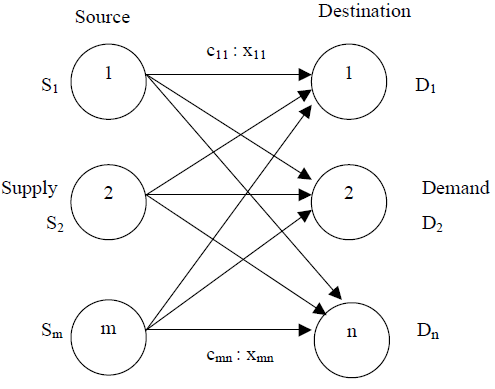
\includegraphics[width=0.46\linewidth]{tt}
		\caption{The Transportation Network}
		\label{fg:3_1}
	\end{figure}
	\begin{figure}[!h]
		\centering
		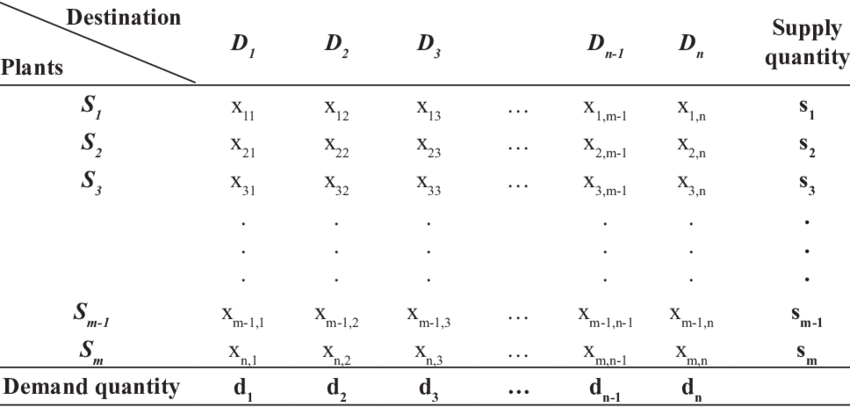
\includegraphics[width=0.65\linewidth]{tt1}
		\caption{The Transportation Tableau}
		\label{fg:3_2}
	\end{figure}
	
	\section{Flowchart Solution of the \tp}
	\begin{itemize}
		\item the problem is formulated as a transportation model
		\item is the transportation model balanced?
		\item if yes, got next step, add dummy to the rows or column
		\item determine initial basic solution
		\item go to next step if the solution is optimized else go to fourth step
		\item using the optimal solution, calculate the total transportation cost
	\end{itemize}
	
	\begin{figure}[!h]
		\centering
		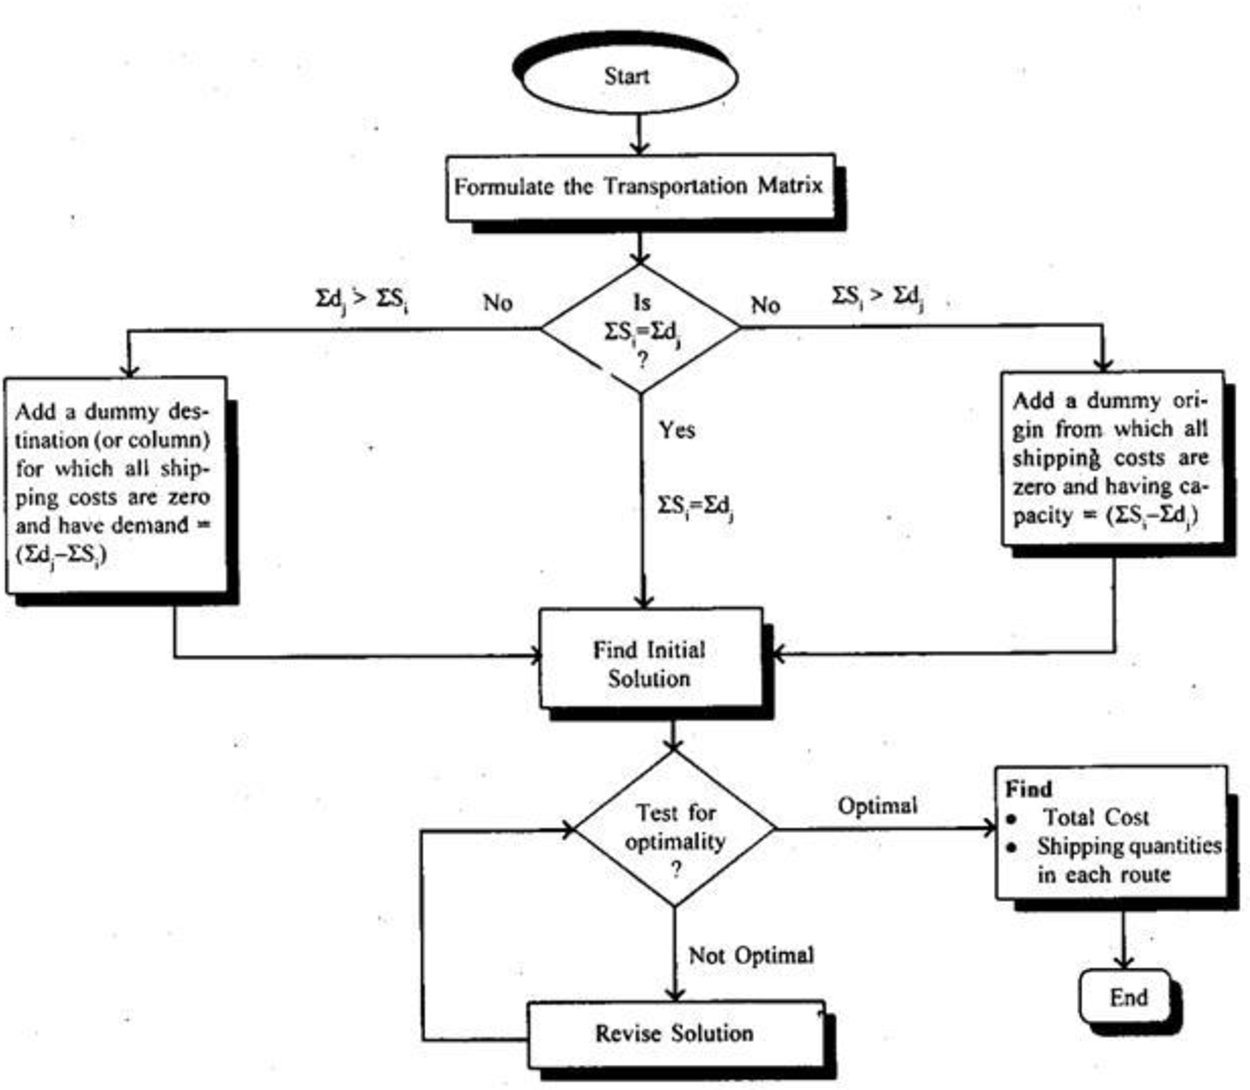
\includegraphics[width=0.7\linewidth]{tt5}
		\caption{Flowchart of Transportation Solution}
		\label{fg:3_3}
	\end{figure}

	\section{Background of Study}
	\subsection{Company Profile}
	The Unilorin Water Enterprise began operations on September 23, 2013, with the promise of producing sparkling clean water for the use of members of the university community and beyond. The Unilorin Water Enterprise is open from Mondays through Saturdays.
	
	\subsection{Company Brand}
	On March 4, 2014, the National Agency for Food and Drug Administration and Control (NAFDAC) approved Unilorin Water Enterprise (UWE) by assigning product registration numbers to the two water brands. Unilorin table water 50cl and 75cl bottles with registration number (1-2090L) and Unilorin Pure water with registration number (1-2049L).
	
	\subsection{Process of Production}
	The factory manufactures and packages the product in a calm and sanitary atmosphere; the company has five sedimentation tanks connected to a particular borehole, huwa-san, sand filter, carbon filter, and four treated water tanks. The business has a micro filter reserve osmosis, treated water tank, ultra violet sterilizer, and washing, filling, and capping equipment for sachet water, and an automatic packaging machine for bottle water.
	
	\subsection{Storehouses}
	The warehouse in the senior staff quarters store house stores raw materials, semi-finished items, and completed goods. This final goods and services are provided on time and at a low cost. There are only three registered transporters in charge of loading, packing, unloading, and moving finished items from the manufacturing warehouse to the distributors.
	
	\subsection{Distributions}
	Finished goods are sold directly to registered distributors. The distributors are the primary agents who distribute to retailers; the university of Ilorin water company produces on a huge scale and has over 70 distributors on and off campus. The firm produces about 4000 bags of sachet water, 500 packs of 50cl Unilorin table water, and 1000 packs of 75cl table water.

	\section{Problem Statement}
	The project will attempt to resolve the challenge of determining the ideal transportation plan that will reduce the overall cost of transporting products from the major production locations to the many important distributors in Ilorin who are geographically dispersed.

	\section{Aim and Objectives}
	\subsection{Aim}
	The Aim of the study is to develop a transportation model of \uwe.
	\subsection{Objectives}
	The study intended:
	\begin{enumerate}
		\renewcommand{\labelenumi}{(\roman{enumi})}
		\item To develop a model of distribution of Unilorin Water Enterprise (UWE) products as a \stp.
		\item To minimize the transportation cost.
		\item To maximize profit.
	\end{enumerate}
	
	
	%%%%%%%%%%%%%%%%%%%%%%%%%CHAPTER TWO%%%%%%%%%%%%%%%%%%%%%%%%%
	\chapter{LITERATURE REVIEW}
	The \stp (TP) is an important Linear Programming (LP) model that arises in several context and has deservingly received much attention in literature.\\
	
	\NI The \stp is probably the most important special linear \stp in terms of relative frequency with which it appears in the applications and also in the simplicity of the procedure developed for its solution. The following features of the transportation problem are considered to be most important.\\
	
	\NI The \stp were the earliest class of Linear Programs discovered to have totally unimodular matrices and integrand extreme points resulting in considerable simplification of the Simplex method.\\
	
	\NI The study of the \stps laid the foundation for further theoretical and algorithmic development of the minimal cost network flow problems.\\
	
	\NI The \stp was formalized by the French mathematician Monges (1781). Major advances were made in the field during World War II by the Soviet/Russian mathematician and Economist Leomd Kantorovich. Consequently, the problem as it is now stated is sometimes known as the Monge-Kantorovich \stp. Kantorovich(1942) published a paper on continuous version of the problem and later with Gavurian, and applied study of the capacitated transportation problem Kantorovich et al (1949).\\
	
	\NI Many scientific disciplines have contributed toward analysing problems associated with the transportation problem, including operation research, Economics, Engineering, Geographic Information Science and Geography. It is explored extensively in the Mathematical Programming and Engineering literatures. Sometimes referred to as the facility location and allocation problem, the transportation optimization problem can be modelled as a large-scale mixed integer linear programming problem.\\
	
	\NI The origin of transportation was first presented by Hitchcock, (1941) also presented a study entitled \textit{`The Distribution of a product from several sources to numerous locations'}, this presentation is considered to be transportation problems. Kropmans, (1947), presented an independent study, not related to Hitchcock's and called \textit{``Optimum utilization of the transportation system"}. These two contributions helped in the development of transportation methods which involve a number of shopping sources and a number of destination. The transportation problem, received this named because many of its applications involve determining how to optimally transport goods.
	
	%%%%%%%%%%%%%%%%%%%%%%%%%CHAPTER THREE%%%%%%%%%%%%%%%%%%%%%%%%%%%%
	\chapter{METHODOLOGY}
	
	\section{Introduction}
	This chapter reviews the proposed solution methodology and approach for handling transportation problem in \uwe. The \stp seeks to minimize the total shipping cost of transporting goods from  $m$ origins (each with a supply $s_i$) to $n$ destinations (each with a demand $d_j$) when the unit shipping cost from an origin $i$, to a destination $j$, is $C_{ij}$.
	
	\section{Mathematical Formulation}
	Supposed a company has $m$ warehouses and $n$ retail outlets. A single product is to be shipped from the warehouse to the outlets. Each warehouse has a given level of supply, and each outlet has a given level of demand. We are also given the transportation cost between every pair of warehouse and outlet, and these cost are assumed to be linear. More explicitly, the assumptions are
	\begin{itemize}
		\item the total supply of products from warehouse $i=a$, where $i=1,2,3,\ldots, m$
		\item the total demand of the products at the outlet $j=b$, where $j=1,2,3,\ldots, n$
		\item the cost of sending one unit of the product from warehouse $i$ to outlet $j$ is equal to $C_{ij}$, where $i=1,2,3,\ldots,m$ and $j=1,2,3,\ldots,n$. The total cost of a shipment is linear in size of shipment.
	\end{itemize}
	

	

	\section{Solution of A \tp}
	\NI \bt{Solving the Transportation Problem:-} There are three popular methods to finding an initial basic feasible solution and they include:
	\begin{enumerate}
		\renewcommand{\labelenumi}{(\arabic{enumi})}
		\item Northwest Corner Rule
		\item Least Cost Method
		\item Vogel Approximation Method
	\end{enumerate}
	
	\subsubsection{Northwest Corner Rule(NCR)} 
	In this method, allocation of quantities being transported from source to some destination must start from the upper most left hand cell that is the Northwest Corner of the table. The steps include:
	\begin{enumerate}
		\renewcommand{\labelenumi}{(\alph{enumi})}
		\item Make allocation in the northwest (upper left) corner of the transportation problem table. Compare the supply of plant 1 say $S_1$ with the demand at the warehouse or destination 1 say $d_1$. Then,
		
		\begin{enumerate}
			\renewcommand{\labelenumii}{(\roman{enumii})}
			\item If $d_1 < S_1$ i.e If the amount required at $d_1$ is less than the number of units available at $S_1$, set $x_{11}$ equal to $d_{1}$, find the balance supply and demand and proceed horizontally.
			
			\item If $d_1 = S_1$, set $x_{11}$ equal to $d_1$, balance supply and demand and proceed diagonally. Remember to make a zero allocation to the least cost cell in $S_1/d_1$.
			
			\item If $d_1 > S_1$, set $x_{11}$ equal to $S_1$, balance demand and supply and proceed vertically.
		\end{enumerate}
	
		\item Continue with $i to iii$, step by step away from the upper left corner until you reach a value in the South-East corner.
		
		\item calculate the total transportation cost.
	\end{enumerate}
	This method does not take into account the transportation cost and hence may not yield a good initial basic feasible solution.
	
	\subsubsection{Least Cost Method (LCM)}
	The Least Cost Method is also called the Matrix Minimum Method, is a method of finding an initial basic feasible solution where allocation of resources begins from the least cost. The steps includes:
	\begin{enumerate}
		\item Determine the cell having the least transportation cost ($C_{ij}$)
		
		\item Allocate as much as possible to this least cost
		
		\item If there's a tie in least cost, select the cell having the greatest least cost.
		
		\item Delete the row or column which has been exhausted
		
		\item Select the next least cost and allocate as much as possible
		
		\item Continue this manner till all row and column requirements are met.
	\end{enumerate}
	
	\subsubsection{The Vogel Approximation Method(VAM)}
	This procedure is an iterative method of finding an initial basic feasible solution. It is an improved version of the least cost method. The steps include:
	\begin{enumerate}
		\item Find the difference between the least cost and next least cost of each row and column(This difference is the row or column penalty).
		
		\item Select the row or column with the biggest penalty
		
		\item In case of a tie in penalty, select the row or column with the greatest least cost
		
		\item Make allocation as much as possible to the cell in that row/column
		
		\item Delete the column or row that has been completely exhausted.
		
		\item Repeat steps 1 to 5 until all allocation are made
	\end{enumerate}
	
	\subsection{Numerical Illustration}
	Consider A company which has 3 production facilities $S_1, S_2$ and $S_3$ with production capacity of $7,9$ and $18$ units(in 100's) per week of a product, respectively. These units are to be shipped to 4 warehouses $D_1, D_2, D_3$ and $D_4$ with requirement of $5, 8, 7$ and $14$ units (in 100's) per week, respectively. The transportation costs (in rupees) per units between factories to warehouse are given in the table below
	
	\begin{table}[h!]
		\centering
		\begin{tabular}{|>{\centering\arraybackslash}m{2.1cm}|>{\centering\arraybackslash}m{1.1cm}|>{\centering\arraybackslash}m{1.1cm}|>{\centering\arraybackslash}m{1.1cm}|>{\centering\arraybackslash}m{1.1cm}||>{\centering\arraybackslash}m{2.7cm}|}
		\hline
			& $D_1$ & $D_2$ & $D_3$ & $D_4$ & Capacity\\\hline
			$S_1$ & 19 & 30 & 50 & 10 & 7\\\hline
			$S_2$ & 70 & 30 & 40 & 60 & 9\\\hline
			$S_3$ & 40 & 8 & 70 & 20 & 18\\\hhline{|=|=|=|=|=#=|}
			Demand & 5 & 8 & 7 & 14 & 34 \\\hline
		\end{tabular}
	\end{table}
	
	\NI To find an initial basic feasible solution for the given transportation problem. Using the three method.\\
	
	\subsection{METHOD 1: Using North West Corner}
	TOTAL number of supply constraints: 3\\
	TOTAL number of demand constraints: 4\\
	\NI Problem Table is
	\begin{longtable}{|>{\centering\arraybackslash}m{2.1cm}|>{\centering\arraybackslash}m{1.1cm}|>{\centering\arraybackslash}m{1.1cm}|>{\centering\arraybackslash}m{1.1cm}|>{\centering\arraybackslash}m{1.1cm}||>{\centering\arraybackslash}m{2.7cm}|}
		\hline
		& $D_1$ & $D_2$ & $D_3$ & $D_4$ & Capacity\\\hline
		$S_1$ & 19 & 30 & 50 & 10 & 7\\\hline
		$S_2$ & 70 & 30 & 40 & 60 & 9\\\hline
		$S_3$ & 40 & 8 & 70 & 20 & 18\\\hhline{|=|=|=|=|=#=|}
		Demand & 5 & 8 & 7 & 14 & 34 \\\hline
	\end{longtable}
	~\\[-1cm]
	\NI The rim values for $S_1 = 7$ and $D_1=5$ are compared\\
	The smaller of the two i.e $\min(7,5) = 5$ is assigned to $S_1D_1$.\\
	This meets the complete demand of $D_1$ and leaves $7-5=2$ units with $S_1$.
	
	~Table-1
	\begin{longtable}{|>{\centering\arraybackslash}m{2.1cm}|>{\centering\arraybackslash}m{1.1cm}|>{\centering\arraybackslash}m{1.1cm}|>{\centering\arraybackslash}m{1.1cm}|>{\centering\arraybackslash}m{1.1cm}||>{\centering\arraybackslash}m{2.7cm}|}
	\hline
		& \tikzmark{a}$D_1$ & $D_2$ & $D_3$ & $D_4$ & Capacity\\\hline
		$S_1$ & 19(5) & 30 & 50 & 10 & 2\\\hline
		$S_2$ & 70 & 30 & 40 & 60 & 9\\\hline
		$S_3$ & \tikzmark{b}40 & 8 & 70 & 20 & 18\\\hhline{|=|=|=|=|=#=|}
		Demand & 0 & 8 & 7 & 14 &  \\\hline
	\end{longtable}
	\linkV{a}{b}
	
	\NI The rim values for $S_1 = 2$ and $D_2=8$ are compared.\\
	The smaller of the two i.e $\min(2,8)=2$ is assigned to $S_1D_2$
	
	\newpage
	~Table-2
	\begin{longtable}{|>{\centering\arraybackslash}m{2.1cm}|>{\centering\arraybackslash}m{1.1cm}|>{\centering\arraybackslash}m{1.1cm}|>{\centering\arraybackslash}m{1.1cm}|>{\centering\arraybackslash}m{1.1cm}||>{\centering\arraybackslash}m{2.7cm}|}
		\hline
		& \tikzmark{aa}$D_1$ & $D_2$ & $D_3$ & $D_4$ & Capacity\\\hline
		\tikzmark{c}$S_1$ & 19(5) & 30(2) & 50 & \tikzmark{d}10 & 0\\\hline
		$S_2$ & 70 & 30 & 40 & 60 & 9\\\hline
		$S_3$ & \tikzmark{bb}40 & 8 & 70 & 20 & 18\\\hhline{|=|=|=|=|=#=|}
		Demand & 0 & 6 & 7 & 14 &  \\\hline
	\end{longtable}
	\linkH{c}{d} \linkV{aa}{bb}
	{~}\\[-1cm]
	\NI The rim value for $S_2 =9$ and $D_2=6$ are compared\\
	The smaller of the two i.e $\min(9,6)=6$ is assigned to $S_2D_2$.\\
	This exhausts the capacity of $S_1$ and leaves $8-2=6$ units with $D_2$
	
	~Table-3
	\begin{longtable}{|>{\centering\arraybackslash}m{2.1cm}|>{\centering\arraybackslash}m{1.1cm}|>{\centering\arraybackslash}m{1.1cm}|>{\centering\arraybackslash}m{1.1cm}|>{\centering\arraybackslash}m{1.1cm}||>{\centering\arraybackslash}m{2.7cm}|}
		\hline
		& \tikzmark{aaa}$D_1$ & \tikzmark{e}$D_2$ & $D_3$ & $D_4$ & Capacity\\\hline
		\tikzmark{cc}$S_1$ & 19(5) & 30(2) & 50 & \tikzmark{dd}10 & 0\\\hline
		$S_2$ & 70 & 30(6) & 40 & 60 & 3\\\hline
		$S_3$ & \tikzmark{bbb}40 & \tikzmark{f}8 & 70 & 20 & 18\\\hhline{|=|=|=|=|=#=|}
		Demand & 0 & 0 & 7 & 14 &  \\\hline
	\end{longtable}
	\linkH{cc}{dd} \linkV{aaa}{bbb} \linkVV{e}{f}{2.5}{1.2}
	{~}\\[-1cm]
	\NI The rim values for $S_2 = 3$ and $D_3=7$ are compared.\\
	The smaller of the two i.e $\min(3,7)=3$ is assigned to $S_2D_3$.
	This exhausts the capacity of $S_2$ and leaves $7-3=4$ units with $D_3$
	\newpage
	~Table-4
	\begin{longtable}{|>{\centering\arraybackslash}m{2.1cm}|>{\centering\arraybackslash}m{1.1cm}|>{\centering\arraybackslash}m{1.1cm}|>{\centering\arraybackslash}m{1.1cm}|>{\centering\arraybackslash}m{1.1cm}||>{\centering\arraybackslash}m{2.7cm}|}
		\hline
		& \tikzmark{aaaa}$D_1$ & \tikzmark{ee}$D_2$ & $D_3$ & $D_4$ & Capacity\\\hline
		\tikzmark{ccc}$S_1$ & 19(5) & 30(2) & 50 & \tikzmark{ddd}10 & 0\\\hline
		\tikzmark{g}$S_2$ & 70 & 30(6) & 40(3) & \tikzmark{h}60 & 0\\\hline
		$S_3$ & \tikzmark{bbbb}40 & \tikzmark{ff}8 & 70 & 20 & 18\\\hhline{|=|=|=|=|=#=|}
		Demand & 0 & 0 & 4 & 14 &  \\\hline
	\end{longtable}
	\linkH{ccc}{ddd} \linkH{g}{h} \linkV{aaaa}{bbbb} \linkVV{ee}{ff}{2.5}{1.2}
	{~}\\[-1cm]
	\NI The rim values for $S_3 = 18$ and $D_3=4$ are compared\\
	This smaller of the two i.e $\min(18,4)=4$ is assigned to $S_3D_3$\\
	This meets the complete demands of $D_3$ and leaves $18-4=14$ units with $S_3$.
	
	~Table-5
	\begin{longtable}{|>{\centering\arraybackslash}m{2.1cm}|>{\centering\arraybackslash}m{1.1cm}|>{\centering\arraybackslash}m{1.1cm}|>{\centering\arraybackslash}m{1.1cm}|>{\centering\arraybackslash}m{1.1cm}||>{\centering\arraybackslash}m{2.7cm}|}
		\hline
		& \tikzmark{aaaaa}$D_1$ & \tikzmark{eee}$D_2$ & \tikzmark{i}$D_3$ & $D_4$ & Capacity\\\hline
		\tikzmark{cccc}$S_1$ & 19(5) & 30(2) & 50 & \tikzmark{dddd}10 & 0\\\hline
		\tikzmark{gg}$S_2$ & 70 & 30(6) & 40(3) & \tikzmark{hh}60 & 0\\\hline
		$S_3$ & \tikzmark{bbbbb}40 & \tikzmark{fff}8 & \tikzmark{j}70(4) & 20 & 14\\\hhline{|=|=|=|=|=#=|}
		Demand & 0 & 0 & 0 & 14 &  \\\hline
	\end{longtable}
	\linkH{cccc}{dddd} \linkH{gg}{hh} \linkV{aaaaa}{bbbbb} \linkVV{eee}{fff}{2.5}{1.2}\linkVV{i}{j}{2.5}{4.2}
	{~}\\[-1cm]
	\NI The rim values for $S_3 = 14$ and $D_4=14$ are compared.\\
	The smaller of the two i.e $\min(14,14)=14$ is assigned to $S_3D_4$
	
	\newpage
	~Table-6
	\begin{longtable}{|>{\centering\arraybackslash}m{2.1cm}|>{\centering\arraybackslash}m{1.1cm}|>{\centering\arraybackslash}m{1.1cm}|>{\centering\arraybackslash}m{1.1cm}|>{\centering\arraybackslash}m{1.1cm}||>{\centering\arraybackslash}m{2.7cm}|}
		\hline
		& \tikzmark{aaaaaa}$D_1$ & \tikzmark{eeee}$D_2$ & \tikzmark{ii}$D_3$ & $D_4$ & Capacity\\\hline
		\tikzmark{ccccc}$S_1$ & 19(5) & 30(2) & 50 & \tikzmark{ddddd}10 & 0\\\hline
		\tikzmark{ggg}$S_2$ & 70 & 30(6) & 40(3) & \tikzmark{hhh}60 & 0\\\hline
		\tikzmark{k}$S_3$ & \tikzmark{bbbbbb}40 & \tikzmark{ffff}8 & \tikzmark{jj}70(4) & \tikzmark{l}20(14) & 0\\\hhline{|=|=|=|=|=#=|}
		Demand & 0 & 0 & 0 & 0 &  \\\hline
	\end{longtable}
	\linkH{ccccc}{ddddd} \linkH{ggg}{hhh} \linkH{k}{l} \linkV{aaaaaa}{bbbbbb} \linkVV{eeee}{ffff}{2.5}{1.2}\linkVV{ii}{jj}{2.5}{4.2}
	{~}\\[-1cm]
	~Initial feasible solution is
	\begin{longtable}{|>{\centering\arraybackslash}m{2.1cm}|>{\centering\arraybackslash}m{1.1cm}|>{\centering\arraybackslash}m{1.1cm}|>{\centering\arraybackslash}m{1.1cm}|>{\centering\arraybackslash}m{1.1cm}||>{\centering\arraybackslash}m{2.7cm}|}
		\hline
		& $D_1$ &$D_2$ & $D_3$ & $D_4$ & Capacity\\\hline
		$S_1$ & 19(5) & 30(2) & 50 & 10 & 7\\\hline
		$S_2$ & 70 & 30(6) & 40(3) & 60 & 9\\\hline
		$S_3$ & 40 & 8 &70(4) & 20(14) & 18\\\hhline{|=|=|=|=|=#=|}
		Demand & 5 & 8 & 7 & 14 &  \\\hline
	\end{longtable}
	
	\NI The minimum total transportation cost
	\begin{gather*}
		19 \times 5 + 30 \times 2 + 30 \times 6 + + 40 \times 3 + 70 \times 4 + 20 \times 14 = 1015 \\[-1cm]
	\end{gather*}
	Here, the number of allocated cells = 6 is equal to 
	\begin{gather*}
	m+n-1 = 3+4-1 = 6\\[-1.2cm]
	\end{gather*}
	$\therefore$ This solution is non-degenerate
	
	
	\subsection{METHOD 2: Using Least Cost Method to find solution}
	TOTAL number of supply constraints: 3\\
	TOTAL number of demand constraints: 4\\
	{~}\\[-0.5cm]
	\NI Problem Table is
	\begin{longtable}{|>{\centering\arraybackslash}m{2.1cm}|>{\centering\arraybackslash}m{1.1cm}|>{\centering\arraybackslash}m{1.1cm}|>{\centering\arraybackslash}m{1.1cm}|>{\centering\arraybackslash}m{1.1cm}||>{\centering\arraybackslash}m{2.7cm}|}
		\hline
		& $D_1$ & $D_2$ & $D_3$ & $D_4$ & Capacity\\\hline
		$S_1$ & 19 & 30 & 50 & 10 & 7\\\hline
		$S_2$ & 70 & 30 & 40 & 60 & 9\\\hline
		$S_3$ & 40 & 8 & 70 & 20 & 18\\\hhline{|=|=|=|=|=#=|}
		Demand & 5 & 8 & 7 & 14 &  \\\hline
	\end{longtable}
	{~}\\[-1cm]
	\NI The smallest transportation cost is $8$ in cell $S_3D_2$\\
	The allocation to this cell is $\min(18,8)=8$\\
	This satisfies the entire demand of $D_2$ and leaves $18-8=10$ units with $S_3$\\
	
	~Table-1
	\begin{longtable}{|>{\centering\arraybackslash}m{2.1cm}|>{\centering\arraybackslash}m{1.1cm}|>{\centering\arraybackslash}m{1.1cm}|>{\centering\arraybackslash}m{1.1cm}|>{\centering\arraybackslash}m{1.1cm}||>{\centering\arraybackslash}m{2.7cm}|}
		\hline
		& $D_1$ & \tikzmark{a0}$D_2$ & $D_3$ & $D_4$ & Capacity\\\hline
		$S_1$ & 19 & 30 & 50 & 10 & 7\\\hline
		$S_2$ & 70 & 30 & 40 & 60 & 9\\\hline
		$S_3$ & 40 & \tikzmark{a1}8(8) & 70 & 20 & 10\\\hhline{|=|=|=|=|=#=|}
		Demand & 5 & 0 & 7 & 14 &  \\\hline
	\end{longtable}
	\linkVV{a0}{a1}{2.5}{3.5}
	{~}\\[-1cm]
	\NI The smallest transportation cost is $10$ in cell $S_1D_4$\\
	The allocation to this is $\min(7,14)=7$\\
	The exhausts the capacity of $S_1$ and leaves $14-7=7$ units with $D_4$
	
	~Table-2
	\begin{longtable}{|>{\centering\arraybackslash}m{2.1cm}|>{\centering\arraybackslash}m{1.1cm}|>{\centering\arraybackslash}m{1.1cm}|>{\centering\arraybackslash}m{1.1cm}|>{\centering\arraybackslash}m{1.1cm}||>{\centering\arraybackslash}m{2.7cm}|}
		\hline
		& $D_1$ & \tikzmark{a2}$D_2$ & $D_3$ & $D_4$ & Capacity\\\hline
		\tikzmark{b0}$S_1$ & 19 & 30 & 50 & \tikzmark{b1}10(7) & 0\\\hline
		$S_2$ & 70 & 30 & 40 & 60 & 9\\\hline
		$S_3$ & 40 & \tikzmark{a3}8(8) & 70 & 20 & 10\\\hhline{|=|=|=|=|=#=|}
		Demand & 5 & 0 & 7 & 7 &  \\\hline
	\end{longtable}
	\linkVV{a2}{a3}{2.5}{3.5}\linkH{b0}{b1}
	{~}\\[-1cm]
	\NI The smallest transportation cost is $20$ in cell $S_3D_4$\\
	The allocation of the cell is $\min(10,7)=7$\\
	This satisfies the entire demand of $D_4$ and leaves $10-7=3$ units with $S_3$\\
	
	~Table-3
	\begin{longtable}{|>{\centering\arraybackslash}m{2.1cm}|>{\centering\arraybackslash}m{1.1cm}|>{\centering\arraybackslash}m{1.1cm}|>{\centering\arraybackslash}m{1.1cm}|>{\centering\arraybackslash}m{1.1cm}||>{\centering\arraybackslash}m{2.7cm}|}
		\hline
		& $D_1$ & \tikzmark{a4}$D_2$ & $D_3$ & \tikzmark{c0}$D_4$ & Capacity\\\hline
		\tikzmark{b2}$S_1$ & 19 & 30 & 50 & \tikzmark{b3}10(7) & 0\\\hline
		$S_2$ & 70 & 30 & 40 & 60 & 9\\\hline
		$S_3$ & 40 & \tikzmark{a5}8(8) & 70 & \tikzmark{c1}20(7) & 3\\\hhline{|=|=|=|=|=#=|}
		Demand & 5 & 0 & 7 & 0 &  \\\hline
	\end{longtable}
	\linkVV{a4}{a5}{2.5}{3.5}\linkH{b2}{b3}\linkVV{c0}{c1}{2.5}{3.5}
	{~}\\[-1.6cm]
	
	\NI The smallest transportation cost is $40$ in cell $S_2D_3$\\
	The allocation to this cell is $\min(9,7)=7$\\
	This satisfies the entire demand of $D_3$ and leaves $9-7=2$ units with $S_2$\\
	\newpage
	~Table-4
	\begin{longtable}{|>{\centering\arraybackslash}m{2.1cm}|>{\centering\arraybackslash}m{1.1cm}|>{\centering\arraybackslash}m{1.1cm}|>{\centering\arraybackslash}m{1.1cm}|>{\centering\arraybackslash}m{1.1cm}||>{\centering\arraybackslash}m{2.7cm}|}
		\hline
		& $D_1$ & \tikzmark{a6}$D_2$ &\tikzmark{d0} $D_3$ & \tikzmark{c2}$D_4$ & Capacity\\\hline
		\tikzmark{b4}$S_1$ & 19 & 30 & 50 & \tikzmark{b5}10(7) & 0\\\hline
		$S_2$ & 70 & 30 & 40(7) & 60 & 2\\\hline
		$S_3$ & 40 & \tikzmark{a7}8(8) & \tikzmark{d1}70 & \tikzmark{c3}20(7) & 3\\\hhline{|=|=|=|=|=#=|}
		Demand & 5 & 0 & 0 & 0 &  \\\hline
	\end{longtable}
	\linkVV{a6}{a7}{2.5}{3.5}\linkH{b4}{b5}\linkVV{c2}{c3}{2.5}{3.5}\linkVV{d0}{d1}{3.5}{2.5}
	{~}\\[-1.6cm]
	
	\NI The smallest transportation cost is $40$ in cell $S_3D_1$\\
	The allocation to this cell is $\min(3,5)=3$\\
	This exhausts the capacity of $S_3$ and leaves $5-2=2$ units with $D_1$\\
	
	~Table-5
	\begin{longtable}{|>{\centering\arraybackslash}m{2.1cm}|>{\centering\arraybackslash}m{1.1cm}|>{\centering\arraybackslash}m{1.1cm}|>{\centering\arraybackslash}m{1.1cm}|>{\centering\arraybackslash}m{1.1cm}||>{\centering\arraybackslash}m{2.7cm}|}
		\hline
		& $D_1$ & \tikzmark{a8}$D_2$ &\tikzmark{d2} $D_3$ & \tikzmark{c4}$D_4$ & Capacity\\\hline
		\tikzmark{b6}$S_1$ & 19 & 30 & 50 & \tikzmark{b7}10(7) & 0\\\hline
		$S_2$ & 70 & 30 & 40(7) & 60 & 2\\\hline
		\tikzmark{e0}$S_3$ & 40(3) & \tikzmark{a9}8(8) & \tikzmark{d3}70 & \tikzmark{c5}20(7) & 0\\\hhline{|=|=|=|=|=#=|}
		Demand & 2 & 0 & 0 & 0 &  \\\hline
	\end{longtable}
	\linkVV{a8}{a9}{2.5}{3.5}\linkH{b6}{b7}\linkVV{c4}{c5}{2.5}{3.5}\linkVV{d2}{d3}{3.5}{2.5}\linkH{e0}{c5}
	{~}\\[-1.6cm]
	
	\NI The smallest transportation cost is $70$ in cell $S_2D_1$\\
	The allocation to this cell is $\min(2,2)=2$\\
	
	\newpage
	~Table-6
	\begin{longtable}{|>{\centering\arraybackslash}m{2.1cm}|>{\centering\arraybackslash}m{1.1cm}|>{\centering\arraybackslash}m{1.1cm}|>{\centering\arraybackslash}m{1.1cm}|>{\centering\arraybackslash}m{1.1cm}||>{\centering\arraybackslash}m{2.7cm}|}
		\hline
		& $D_1$ & \tikzmark{a10}$D_2$ &\tikzmark{d4} $D_3$ & \tikzmark{c6}$D_4$ & Capacity\\\hline
		\tikzmark{b8}$S_1$ & 19 & 30 & 50 & \tikzmark{b9}10(7) & 0\\\hline
		\tikzmark{f0}$S_2$ & 70(2) & 30 & 40(7) & \tikzmark{f1}60 & 0\\\hline
		\tikzmark{e1}$S_3$ & 40(3) & \tikzmark{a11}8(8) & \tikzmark{d5}70 & \tikzmark{c7}20(7) & 0\\\hhline{|=|=|=|=|=#=|}
		Demand & 0 & 0 & 0 & 0 &  \\\hline
	\end{longtable}
	\linkVV{a10}{a11}{2.5}{3.5}\linkH{b8}{b9}\linkVV{c6}{c7}{2.5}{3.5}\linkVV{d4}{d5}{3.5}{2.5}\linkH{e1}{c7}\linkH{f0}{f1}
	{~}\\[-1.6cm]
	
	~Initial feasible solution is
	\begin{longtable}{|>{\centering\arraybackslash}m{2.1cm}|>{\centering\arraybackslash}m{1.1cm}|>{\centering\arraybackslash}m{1.1cm}|>{\centering\arraybackslash}m{1.1cm}|>{\centering\arraybackslash}m{1.1cm}||>{\centering\arraybackslash}m{2.7cm}|}
		\hline
		& $D_1$ & $D_2$ &{d4} $D_3$ & $D_4$ & Capacity\\\hline
		$S_1$ & 19 & 30 & 50 & 10(7) & 7\\\hline
		$S_2$ & 70(2) & 30 & 40(7) & 60 & 9\\\hline
		$S_3$ & 40(3) & 8(8) & 70 & 20(7) & 18\\\hhline{|=|=|=|=|=#=|}
		Demand & 5 & 8 & 7 & 14 &  \\\hline
	\end{longtable}
	
	\NI The minimum total transportation cost
	\begin{gather*}
		10 \times 7 + 70 \times 2 + 40 \times 3 + 8 \times 8 + 20 \times 7 = 814 \\[-1cm]
	\end{gather*}
	Here, the number of allocated cells = 6 is equal to 
	\begin{gather*}
		m+n-1 = 3+4-1 = 6\\[-1.2cm]
	\end{gather*}
	$\therefore$ This solution is non-degenerate
	
	
	\subsection{METHOD 3: Using Vogel's Approximation Method to find solution}
	TOTAL number of supply constraints: 3\\
	TOTAL number of demand constraints: 4\\
	{~}\\[-0.5cm]
	\NI Problem Table is
	\begin{longtable}{|>{\centering\arraybackslash}m{2.1cm}|>{\centering\arraybackslash}m{1.1cm}|>{\centering\arraybackslash}m{1.1cm}|>{\centering\arraybackslash}m{1.1cm}|>{\centering\arraybackslash}m{1.1cm}||>{\centering\arraybackslash}m{2.7cm}|}
		\hline
		& $D_1$ & $D_2$ & $D_3$ & $D_4$ & Capacity\\\hline
		$S_1$ & 19 & 30 & 50 & 10 & 7\\\hline
		$S_2$ & 70 & 30 & 40 & 60 & 9\\\hline
		$S_3$ & 40 & 8 & 70 & 20 & 18\\\hhline{|=|=|=|=|=#=|}
		Demand & 5 & 8 & 7 & 14 &  \\\hline
	\end{longtable}
	{~}\\[-1.3cm]
	
	\NI Table-1
	\begin{longtable}{|>{\centering\arraybackslash}m{1.37cm}|>{\centering\arraybackslash}m{1.95cm}|>{\centering\arraybackslash}m{1.7cm}|>{\centering\arraybackslash}m{1.7cm}|>{\centering\arraybackslash}m{1.7cm}||>{\centering\arraybackslash}m{1.47cm}|m{2.2cm}|}
		\hline
		& $D_1$ & $D_2$ & $D_3$ & $D_4$ & Capacity & Row Penalty\\\hline
		$S_1$ & 19 & 30 & 50 & 10 & 7 & 9=19-10\\\hline
		$S_2$ & 70 & 30 & 40 & 60 & 9& 10 = 40-30\\\hline
		$S_3$ & 40 & 8 & 70 & 20 & 18 & 12 = 20-8\\\hhline{|=|=|=|=|=#=|=|}
		Demand & 5 & 8 & 7 & 14 & & \\\hline
		Column Penalty & 21 = 40-19 & 22=30-8 & 10=50-40 & 10=20-10 & &\\\hline
	\end{longtable}
	{~}\\[-1cm]
	The maximum penalty, 22 occur in column $D_2$\\
	The minimum $C_{ij}$ in this column is $C_{32} = 8$\\
	The maximum allocation in this cell is $\min(18,8)=8$\\
	It satisfy demand of $D_2$ and adjust the supply of $S_3$ from 18 to 10 ($18-8=10$).\\
	
	\NI Table-2
	\begin{longtable}{|>{\centering\arraybackslash}m{1.37cm}|>{\centering\arraybackslash}m{1.95cm}|>{\centering\arraybackslash}m{1.2cm}|>{\centering\arraybackslash}m{1.85cm}|>{\centering\arraybackslash}m{1.85cm}||>{\centering\arraybackslash}m{1.47cm}|m{2.2cm}|}
		\hline
		& $D_1$ & \tikzmark{aa0}$D_2$ & $D_3$ & $D_4$ & Capacity & Row Penalty\\\hline
		$S_1$ & 19 & 30 & 50 & 10 & 7 & 9=19-10\\\hline
		$S_2$ & 70 & 30 & 40 & 60 & 9& 20 = 60-40\\\hline
		$S_3$ & 40 & \tikzmark{aa1}8(8) & 70 & 20 & 10 & 20 = 40-20\\\hhline{|=|=|=|=|=#=|=|}
		Demand & 5 & 0 & 7 & 14 & & \\\hline
		Column Penalty & 21 = 40-19 & -- & 10=50-40 & 10=20-10 & &\\\hline
	\end{longtable}
	\linkVV{aa0}{aa1}{2.5}{3.5}
	
	\NI The maximum penalty, 21, occur in column $D_1$\\
	The minimum $C_{ij}$ in this column is $C_{11}=19$\\
	The maximum allocation in this cell is $\min(7,5)=5$\\
	It satisfy demand of $D_1$ and adjust the supply of $S_1$ from 7 to 2 ($7-5=2$)
	
	
	\newpage
	\NI Table-3
	\begin{longtable}{|>{\centering\arraybackslash}m{1.37cm}|>{\centering\arraybackslash}m{1.5cm}|>{\centering\arraybackslash}m{1.5cm}|>{\centering\arraybackslash}m{1.8cm}|>{\centering\arraybackslash}m{1.8cm}||>{\centering\arraybackslash}m{1.47cm}|m{2.2cm}|}
		\hline
		& \tikzmark{bb0}$D_1$ & \tikzmark{aa2}$D_2$ & $D_3$ & $D_4$ & Capacity & Row Penalty\\\hline
		$S_1$ & 19(5) & 30 & 50 & 10 & 2 & 40=50-10\\\hline
		$S_2$ & 70 & 30 & 40 & 60 & 9& 20 = 60-40\\\hline
		$S_3$ & \tikzmark{bb1}40 &  \tikzmark{aa3}8(8) & 70 & 20 & 10 & 50 = 70-20\\\hhline{|=|=|=|=|=#=|=|}
		Demand & 0 & 0 & 7 & 14 & & \\\hline
		Column Penalty & -- & -- & 10=50-40 & 10=20-10 & &\\\hline
	\end{longtable}
	\linkVV{aa2}{aa3}{2.5}{3.5}\linkVV{bb0}{bb1}{2.5}{2.7}
	
	\NI The maximum penalty, 50 occurs in row $S_3$\\
	The minimum $C_{ij}$ in this row is $C_{34}=20$\\
	The maximum allocation in this cell is $\min(10,14)=10$\\
	It satisfy supply of $S_3$ and adjust the demand of $D_4$ from 14 to 4 ($14-10=4$).\\[-0.2cm]
	
	\newpage
	\NI Table-4
	\begin{longtable}{|>{\centering\arraybackslash}m{1.37cm}|>{\centering\arraybackslash}m{1.5cm}|>{\centering\arraybackslash}m{1.5cm}|>{\centering\arraybackslash}m{1.8cm}|>{\centering\arraybackslash}m{1.8cm}||>{\centering\arraybackslash}m{1.47cm}|m{2.3cm}|}
		\hline
		& \tikzmark{bb2}$D_1$ & \tikzmark{aa4}$D_2$ & $D_3$ & $D_4$ & Capacity & Row Penalty\\\hline
		$S_1$ & 19(5) & 30 & 50 & 10 & 2 & 40=50-10\\\hline
		$S_2$ & 70 & 30 & 40 & 60 & 9& 20 = 60-40\\\hline
		\tikzmark{cc10}$S_3$ & \tikzmark{bb3}40 &  \tikzmark{aa5}8(8) & 70 & \tikzmark{cc0}20(10) & 0 & --\\\hhline{|=|=|=|=|=#=|=|}
		Demand & 0 & 0 & 7 & 4 & & \\\hline
		Column Penalty & -- & -- & 10=50-40 & 50=60-10 & &\\\hline
	\end{longtable}
	\linkVV{aa4}{aa5}{2.5}{3.5}\linkVV{bb2}{bb3}{2.5}{2.7}\linkH{cc10}{cc0}
	{~}\\[-1cm]
	The maximum penalty, 50, occurs in column $D_4$\\
	The minimum $C_{ij}$ in this column is $C_{14} = 10$\\
	The maximum allocation in this cell is $\min(2,4)=2$\\
	It satisfy supply of $S_1$ and adjust the demand of $D_4$ from 4 to 2 ($4-2=2$).\\[-0.3cm]
	
	\NI Table-5
	\begin{longtable}{|>{\centering\arraybackslash}m{1.37cm}|>{\centering\arraybackslash}m{1.5cm}|>{\centering\arraybackslash}m{1.5cm}|>{\centering\arraybackslash}m{1.5cm}|>{\centering\arraybackslash}m{1.5cm}||>{\centering\arraybackslash}m{1.47cm}|m{2.3cm}|}
		\hline
		& \tikzmark{bb4}$D_1$ & \tikzmark{aa6}$D_2$ & $D_3$ & $D_4$ & Capacity & Row Penalty\\\hline
		\tikzmark{dd0}$S_1$ & 19(5) & 30 & 50 & \tikzmark{dd1}10(2) & 0 & --\\\hline
		$S_2$ & 70 & 30 & 40 & 60 & 9& 20 = 60-40\\\hline
		\tikzmark{cc11}$S_3$ & \tikzmark{bb5}40 &  \tikzmark{aa7}8(8) & 70 & \tikzmark{cc1}20(10) & 0 & --\\\hhline{|=|=|=|=|=#=|=|}
		Demand & 0 & 0 & 7 & 2 & & \\\hline
		Column Penalty & -- & -- & 40 & 60 & &\\\hline
	\end{longtable}
	\linkVV{aa6}{aa7}{2.5}{3.5}\linkVV{bb4}{bb5}{2.5}{2.7}\linkH{cc11}{cc1}\linkH{dd0}{dd1}
	{~}\\[-1cm]
	The maximum penalty, 60, occurs in column $D_4$\\
	the minimum $C_{ij}$ in this column is $C_{24}=60$\\
	The maximum allocation in this cell is $\min(9,2)=2$\\
	It satisfy demand of $D_4$ and adjust the supply of $S_2$ from 9 to 7 ($9-2=7$)\\
	
	\NI Table-6
	\begin{longtable}{|>{\centering\arraybackslash}m{1.37cm}|>{\centering\arraybackslash}m{1.5cm}|>{\centering\arraybackslash}m{1.5cm}|>{\centering\arraybackslash}m{1.5cm}|>{\centering\arraybackslash}m{1.5cm}||>{\centering\arraybackslash}m{1.47cm}|m{2.3cm}|}
		\hline
		& \tikzmark{bb6}$D_1$ & \tikzmark{aa8}$D_2$ & $D_3$ & $D_4$ & Capacity & Row Penalty\\\hline
		\tikzmark{dd2}$S_1$ & 19(5) & 30 & 50 & \tikzmark{dd3}10(2) & 0 & --\\\hline
		$S_2$ & 70 & 30 & 40 & 60(2) & 7& 40\\\hline
		\tikzmark{cc12}$S_3$ & \tikzmark{bb7}40 &  \tikzmark{aa9}8(8) & 70 & \tikzmark{cc2}20(10) & 0 & --\\\hhline{|=|=|=|=|=#=|=|}
		Demand & 0 & 0 & 7 & 0 & & \\\hline
		Column Penalty & -- & -- & 40 & -- & &\\\hline
	\end{longtable}
	\linkVV{aa8}{aa9}{2.5}{3.5}\linkVV{bb6}{bb7}{2.5}{2.7}\linkH{cc12}{cc2}\linkH{dd2}{dd3}
	{~}\\[-1cm]
	The maximum penalty, 40, occurs in row $S_2$\\
	The minimum $C_{ij}$ in this row is $C_{23}=40$\\
	The maximum allocation in this cell is $\min(7,7)=7$\\
	It satisfy supply of $S_2$ and demand of $D_3$
	
	\newpage
	\NI Initial feasible solution is
	\begin{longtable}{|>{\centering\arraybackslash}m{1.37cm}|>{\centering\arraybackslash}m{1.1cm}|>{\centering\arraybackslash}m{1.1cm}|>{\centering\arraybackslash}m{1.1cm}|>{\centering\arraybackslash}m{1.1cm}||>{\centering\arraybackslash}m{1.47cm}|m{3.6cm}|}
		\hline
		& $D_1$ & $D_2$ & $D_3$ & $D_4$ & Capacity & Row Penalty\\\hline
		$S_1$ & 19(5) & 30 & 50 & 10(2) & 7 & $9|9|40|40|$-$|$-$|$\\\hline
		$S_2$ & 70 & 30 & 40 & 60(2) & 9& $10|20|20|20|20|40|$\\\hline
		$S_3$ & 40 & 8(8) & 70 & 20(10) & 18 & $12|20|50|$-$|$-$|$-$|$\\\hhline{|=|=|=|=|=#=|=|}
		Demand & 5 & 8 & 7 & 14 & & \\\hline
		%\multirow{6}{*}{Column\\Penalty} & -- & -- & 40 & -- & &\\\hline
		& 21 & 22 & 10 & 10 & & \\
		& 21 &-- & 10 & 10 &&\\
		& -- & -- & 10 & 10 &&\\
		& -- & -- & 10 & 50 &&\\
		& -- & -- & 40 & 60 &&\\
		& -- & -- & 40 & -- &&\\\hline
	\end{longtable}
	{~}\\[-1.2cm]
	
	\NI The minimum total transportation cost
	\begin{gather*}
		19\times 5 + 10 \times 2 + 40 \times 7 + 60 \times 2 + 8 \times 8 + 20 \times 10 = 779 \\[-1cm]
	\end{gather*}
	Here, the number of allocated cells = 6 is equal to 
	\begin{gather*}
		m+n-1 = 3+4-1 = 6\\[-1.2cm]
	\end{gather*}
	$\therefore$ This solution is non-degenerate
	
	
	
	%%%%%%%%%%%%%%%%%%%%%%%%%CHAPTER FOUR%%%%%%%%%%%%%%%%%%%%%%%%
	\chapter{DATA COLLECTION AND ANALYSIS}
	\section{Data Collection}
	The table below displays a weekly unbalanced transportation problem data from Unilorin Water Enterprise's storehouses: Factory, Consultancy, Business School, and UITH, each. This problem's demand and supply capacity are provided as 400, 150, 100, 200 and 350, 300, 250, 200 (in packs per week), respectively. The transportation costs (in thousand naira) between factories to warehouses are given per week. 
	\newpage
	\begin{longtable}{|>{\arraybackslash}m{3.1cm}|>{\centering\arraybackslash}m{1.1cm}|>{\centering\arraybackslash}m{1.1cm}|>{\centering\arraybackslash}m{1.1cm}|>{\centering\arraybackslash}m{1.1cm}||>{\centering\arraybackslash}m{4cm}|}
			\hline
		& $W_1$ & $W_2$ & $W_3$ & $W_4$ & Supply Capacity$|$Availability\\\hline
		Factory & 5 & 6 & 5 & 7 & 400\\
		Consultancy & 2 & 2 & 3 & 3 & 150\\
		Business School & 5 & 4 & 4 & 3 & 100\\
		Uith & 13 & 12 & 15 & 12 & 200\\\hhline{|=|=|=|=|=#=|}
		Demand & 350 & 300 & 250 & 200 &  \\\hline
	\end{longtable}

	\NI This study covers data collection from the month of September - October, 2021.

	\section{Data Analysis}

	\begin{longtable}{|>{\arraybackslash}m{3.1cm}|>{\centering\arraybackslash}m{1.1cm}|>{\centering\arraybackslash}m{1.1cm}|>{\centering\arraybackslash}m{1.1cm}|>{\centering\arraybackslash}m{1.1cm}||>{\centering\arraybackslash}m{4cm}|}
			\hline
			& $D_1$ & $D_2$ & $D_3$ & $D_4$ & Supply Capacity$|$Availability\\\hline
			Factory & 100 & 50 & 130 & 70 & 200\\
			Consultancy & 90 & 60 & 80 & 100 & 100\\
			Business School & 150 & 20 & 300 & 100 & 300\\
			Uith & 15 & 12 & 24 & 10 & 30\\\hhline{|=|=|=|=|=#=|}
			Demand & 200 & 150 & 150 & 130 & 630 \\\hline
	\end{longtable}

	\NI To find an initial basic feasible solution for the given transportation problem using the three method. Representing the stores as $S_1, S_2, S_3, S_4$.
	
	\section{METHOD 1: Using North West Corner}
	TOTAL number of supply constraints: 4\\
	TOTAL number of demand constraints: 4\\
	\begin{longtable}{|>{\centering\arraybackslash}m{2.1cm}|>{\centering\arraybackslash}m{1.7cm}|>{\centering\arraybackslash}m{1.7cm}|>{\centering\arraybackslash}m{1.7cm}|>{\centering\arraybackslash}m{1.7cm}||>{\centering\arraybackslash}m{2.7cm}|}
		\hline
		& $D_1$ &$D_2$ & $D_3$ & $D_4$ & Supply\\\hline
		$S_1$ & 100 & 50 & 130 & 70 & 200\\
		$S_2$ & 90 & 60 & 80 & 100 & 100\\
		$S_3$ & 150 & 20 & 300 & 100 & 300\\
		$S_4$ &15 & 12 & 24 & 10 & 30\\\hhline{|=|=|=|=|=#=|}
		Demand & 200 & 150 & 150 & 130 &  \\\hline
	\end{longtable}
	\NI The rim values for $S_1=200$ and $D_1=200$ are compared\\
	The smaller of the two i.e $\min(200,200) = 200$ is assigned to $S_1D_1$\\
	This exhausts the capacity of $S_1$ and leaves $200-200=0$ units with $D_1$\\
	
	\NI~Table-1
		\begin{longtable}{|>{\centering\arraybackslash}m{2.1cm}|>{\centering\arraybackslash}m{1.7cm}|>{\centering\arraybackslash}m{1.7cm}|>{\centering\arraybackslash}m{1.7cm}|>{\centering\arraybackslash}m{1.4cm}||>{\centering\arraybackslash}m{2.7cm}|}
		\hline
		& \tikzmark{j1}$D_1$ &$D_2$ & $D_3$ & $D_4$ & Supply\\\hline
		\tikzmark{i1}$S_1$ & 100(200) & 50 & 130 & \tikzmark{i2}70 & 0\\
		$S_2$ & 90 & 60 & 80 & 100 & 100\\
		$S_3$ & 150 & 20 & 300 & 100 & 300\\
		$S_4$ &\tikzmark{j2}15 & 12 & 24 & 10 & 30\\\hhline{|=|=|=|=|=#=|}
		Demand & 0 & 150 & 150 & 130 &  \\\hline
	\end{longtable}
	\linkV{j1}{j2}\linkH{i1}{i2}
	{~}\\[-1cm]
	\NI The rim values for $S_2=100$ and $D_1=0$ are compared\\
	The smaller of the two i.e $\min(100,0) = 0$ is assigned to $S_2D_1$\\
	This meets the complete demands of $D_1$ and leaves $100-0=100$ units with $S_2$\\
	
	\NI~Table-2
	\begin{longtable}{|>{\centering\arraybackslash}m{2.1cm}|>{\centering\arraybackslash}m{1.7cm}|>{\centering\arraybackslash}m{1.7cm}|>{\centering\arraybackslash}m{1.7cm}|>{\centering\arraybackslash}m{1.4cm}||>{\centering\arraybackslash}m{2.7cm}|}
		\hline
		& \tikzmark{j3}$D_1$ &$D_2$ & $D_3$ & $D_4$ & Supply\\\hline
		\tikzmark{i3}$S_1$ & 100(200) & 50 & 130 & \tikzmark{i4}70 & 0\\
		$S_2$ & 90 & 60 & 80 & 100 & 100\\
		$S_3$ & 150 & 20 & 300 & 100 & 300\\
		$S_4$ &\tikzmark{j4}15 & 12 & 24 & 10 & 30\\\hhline{|=|=|=|=|=#=|}
		Demand & 0 & 150 & 150 & 130 &  \\\hline
	\end{longtable}
	\linkV{j3}{j4}\linkH{i3}{i4}
	{~}\\[-1cm]
	\NI The rim values for $S_2=100$ and $D_2=150$ are compared\\
	The smaller of the two i.e $\min(100,150) = 100$ is assigned to $S_2D_2$\\
	This exhaust the capacity of $S_2$ and leaves $150-100=50$ units with $D_2$\\
	
	\NI~Table-3
	\begin{longtable}{|>{\centering\arraybackslash}m{2.1cm}|>{\centering\arraybackslash}m{1.7cm}|>{\centering\arraybackslash}m{1.7cm}|>{\centering\arraybackslash}m{1.7cm}|>{\centering\arraybackslash}m{1.4cm}||>{\centering\arraybackslash}m{2.7cm}|}
		\hline
		& \tikzmark{j5}$D_1$ &$D_2$ & $D_3$ & $D_4$ & Supply\\\hline
		\tikzmark{i5}$S_1$ & 100(200) & 50 & 130 & \tikzmark{i6}70 & 0\\
		\tikzmark{l1}$S_2$ & 90 & 60(100) & 80 & \tikzmark{l2}100 & 0\\
		$S_3$ & 150 & 20 & 300 & 100 & 300\\
		$S_4$ &\tikzmark{j6}15 & 12 & 24 & 10 & 30\\\hhline{|=|=|=|=|=#=|}
		Demand & 0 & 50 & 150 & 130 &  \\\hline
	\end{longtable}
	\linkV{j5}{j6}\linkH{i5}{i6}\linkH{l1}{l2}
	{~}\\[-1cm]
	\NI The rim values for $S_3=300$ and $D_2=50$ are compared\\
	The smaller of the two i.e $\min(300,50) = 50$ is assigned to $S_3D_2$\\
	This meets the complete demand of $D_2$ and leaves $300-50=250$ units with $S_3$\\
	
	\NI~Table-4
	\begin{longtable}{|>{\centering\arraybackslash}m{2.1cm}|>{\centering\arraybackslash}m{1.7cm}|>{\centering\arraybackslash}m{1.7cm}|>{\centering\arraybackslash}m{1.7cm}|>{\centering\arraybackslash}m{1.4cm}||>{\centering\arraybackslash}m{2.7cm}|}
		\hline
		& \tikzmark{j7}$D_1$ &\tikzmark{m1}$D_2$ & $D_3$ & $D_4$ & Supply\\\hline
		\tikzmark{i7}$S_1$ & 100(200) & 50 & 130 & \tikzmark{i8}70 & 0\\
		\tikzmark{l3}$S_2$ & 90 & 60(100) & 80 & \tikzmark{l4}100 & 0\\
		$S_3$ & 150 & 20(50) & 300 & 100 & 250\\
		$S_4$ &\tikzmark{j8}15 & \tikzmark{m2}12 & 24 & 10 & 30\\\hhline{|=|=|=|=|=#=|}
		Demand & 0 & 0 & 150 & 130 &  \\\hline
	\end{longtable}
	\linkV{j7}{j8}\linkH{i7}{i8}\linkH{l3}{l4}\linkV{m1}{m2}
	{~}\\[-1cm]
	\NI The rim values for $S_3=250$ and $D_3=150$ are compared\\
	The smaller of the two i.e $\min(250,150) = 150$ is assigned to $S_3D_3$\\
	This meets the complete demand of $D_3$ and leaves $250-150=100$ units with $S_3$\\
	\newpage
	\NI~Table-5
	\begin{longtable}{|>{\centering\arraybackslash}m{2.1cm}|>{\centering\arraybackslash}m{1.7cm}|>{\centering\arraybackslash}m{1.7cm}|>{\centering\arraybackslash}m{1.7cm}|>{\centering\arraybackslash}m{1.4cm}||>{\centering\arraybackslash}m{2.7cm}|}
		\hline
		& \tikzmark{j9}$D_1$ &\tikzmark{m3}$D_2$ & \tikzmark{n1}$D_3$ & $D_4$ & Supply\\\hline
		\tikzmark{i9}$S_1$ & 100(200) & 50 & 130 & \tikzmark{i10}70 & 0\\
		\tikzmark{l5}$S_2$ & 90 & 60(100) & 80 & \tikzmark{l6}100 & 0\\
		$S_3$ & 150 & 20(50) & 300(150) & 100 & 100\\
		$S_4$ &\tikzmark{j10}15 & \tikzmark{m4}12 & \tikzmark{n2}24 & 10 & 30\\\hhline{|=|=|=|=|=#=|}
		Demand & 0 & 0 & 0 & 130 &  \\\hline
	\end{longtable}
	\linkV{j9}{j10}\linkH{i9}{i10}\linkH{l5}{l6}\linkV{m3}{m4}\linkV{n1}{n2}
	{~}\\[-1cm]
	\NI The rim values for $S_3=100$ and $D_4=130$ are compared\\
	The smaller of the two i.e $\min(100,130) = 100$ is assigned to $S_3D_4$\\
	This exhausts the capacity of $S_3$ and leaves $130-100=30$ units with $D_4$\\
	
	\NI~Table-6
	\begin{longtable}{|>{\centering\arraybackslash}m{2.1cm}|>{\centering\arraybackslash}m{1.7cm}|>{\centering\arraybackslash}m{1.7cm}|>{\centering\arraybackslash}m{1.7cm}|>{\centering\arraybackslash}m{1.4cm}||>{\centering\arraybackslash}m{2.7cm}|}
		\hline
		& \tikzmark{j11}$D_1$ &\tikzmark{m5}$D_2$ & \tikzmark{n3}$D_3$ & $D_4$ & Supply\\\hline
		\tikzmark{i11}$S_1$ & 100(200) & 50 & 130 & \tikzmark{i12}70 & 0\\
		\tikzmark{l7}$S_2$ & 90 & 60(100) & 80 & \tikzmark{l8}100 & 0\\
		\tikzmark{o1}$S_3$ & 150 & 20(50) & 300(150) & \tikzmark{o2}100(100) & 0\\
		$S_4$ &\tikzmark{j12}15 & \tikzmark{m6}12 & \tikzmark{n4}24 & 10 & 30\\\hhline{|=|=|=|=|=#=|}
		Demand & 0 & 0 & 0 & 30 &  \\\hline
	\end{longtable}
	\linkV{j11}{j12}\linkH{i11}{i12}\linkH{l7}{l8}\linkV{m5}{m6}\linkV{n3}{n4}\linkH{o1}{o2}
	{~}\\[-1cm]
	\NI The rim values for $S_4=30$ and $D_4=30$ are compared\\
	The smaller of the two i.e $\min(30,30) = 30$ is assigned to $S_4D_4$\\
	
	
	\NI~Table-7
	\begin{longtable}{|>{\centering\arraybackslash}m{2.1cm}|>{\centering\arraybackslash}m{1.7cm}|>{\centering\arraybackslash}m{1.7cm}|>{\centering\arraybackslash}m{1.7cm}|>{\centering\arraybackslash}m{1.4cm}||>{\centering\arraybackslash}m{2.7cm}|}
		\hline
		& \tikzmark{j13}$D_1$ &\tikzmark{m7}$D_2$ & \tikzmark{n5}$D_3$ & $D_4$ & Supply\\\hline
		\tikzmark{i13}$S_1$ & 100(200) & 50 & 130 & \tikzmark{i14}70 & 0\\
		\tikzmark{l9}$S_2$ & 90 & 60(100) & 80 & \tikzmark{l10}100 & 0\\
		\tikzmark{o3}$S_3$ & 150 & 20(50) & 300(150) & \tikzmark{o4}100(100) & 0\\
		\tikzmark{p1}$S_4$ &\tikzmark{j14}15 & \tikzmark{m8}12 & \tikzmark{n6}24 & \tikzmark{p2}10(30) & 0\\\hhline{|=|=|=|=|=#=|}
		Demand & 0 & 0 & 0 & 0 &  \\\hline
	\end{longtable}
	\linkV{j13}{j14}\linkH{i13}{i14}\linkH{l9}{l10}\linkV{m7}{m8}\linkV{n5}{n6}\linkH{o3}{o4}\linkH{p1}{p2}
	{~}\\[-.6cm]
	\NI Initial feasible solution is
		\begin{longtable}{|>{\centering\arraybackslash}m{2.1cm}|>{\centering\arraybackslash}m{1.7cm}|>{\centering\arraybackslash}m{1.7cm}|>{\centering\arraybackslash}m{1.7cm}|>{\centering\arraybackslash}m{1.4cm}||>{\centering\arraybackslash}m{2.7cm}|}
		\hline
		&$D_1$ &$D_2$ & $D_3$ & $D_4$ & Supply\\\hline
		$S_1$ & 100(200) & 50 & 130 & 70 & 200\\
		$S_2$ & 90 & 60(100) & 80 & 100 & 100\\
		$S_3$ & 150 & 20(50) & 300(150) & 100(100) & 300\\
		$S_4$ &15 & 12 & 24 & 10(30) & 30\\\hhline{|=|=|=|=|=#=|}
		Demand & 200 & 150 & 150 & 130 &  \\\hline
	\end{longtable}
	
	\NI The minimum total transportation cost 
		\begin{gather*}
			100\times 200 + 60 \times 100 | 20 \times 50 + 300 \times 150 + 100\times 100 + 10\times 30 = 82000
		\end{gather*}
	 
	\NI Here, the number of allocated cells = 6 which is one less than to
	\begin{gather*}
		m+n-1 = 4+4-1 = 7
	\end{gather*}
	$\therefore$ the solution is degenerate.
	
	\section{METHOD 2: Using Least Cost}
	TOTAL number of supply constraints: 4\\
	TOTAL number of demand constraints: 4\\
	Problem Table is\\[-.8cm]
	\begin{longtable}{|>{\centering\arraybackslash}m{2.1cm}|>{\centering\arraybackslash}m{1.7cm}|>{\centering\arraybackslash}m{1.7cm}|>{\centering\arraybackslash}m{1.7cm}|>{\centering\arraybackslash}m{1.7cm}||>{\centering\arraybackslash}m{2.7cm}|}
		\hline
		& $D_1$ &$D_2$ & $D_3$ & $D_4$ & Supply\\\hline
		$S_1$ & 100 & 50 & 130 & 70 & 200\\
		$S_2$ & 90 & 60 & 80 & 100 & 100\\
		$S_3$ & 150 & 20 & 300 & 100 & 300\\
		$S_4$ &15 & 12 & 24 & 10 & 30\\\hhline{|=|=|=|=|=#=|}
		Demand & 200 & 150 & 150 & 130 &  \\\hline
	\end{longtable}
	~\\[-1.2cm]
	\NI The smallest transportation cost  is 10 in cell $S_4D_4$\\
	The allocation to this cell is $\min(30,130)=30$\\
	This exhausts the capacity of $S_4$ and leaves $130-30=100$ units with $D_4$\\[-.4cm]
	
	\NI Table 1\\[-.8cm]
	\begin{longtable}{|>{\centering\arraybackslash}m{2.1cm}|>{\centering\arraybackslash}m{1.7cm}|>{\centering\arraybackslash}m{1.7cm}|>{\centering\arraybackslash}m{1.7cm}|>{\centering\arraybackslash}m{1.7cm}||>{\centering\arraybackslash}m{2.7cm}|}
		\hline
		& $D_1$ &$D_2$ & $D_3$ & $D_4$ & Supply\\\hline
		$S_1$ & 100 & 50 & 130 & 70 & 200\\
		$S_2$ & 90 & 60 & 80 & 100 & 100\\
		$S_3$ & 150 & 20 & 300 & 100 & 300\\
		\tikzmark{q1}$S_4$ &15 & 12 & 24 & \tikzmark{q2}10(30) & 0\\\hhline{|=|=|=|=|=#=|}
		Demand & 200 & 150 & 150 & 100 &  \\\hline
	\end{longtable}
	\linkH{q1}{q2}
	~\\[-1.1cm]
	\NI The smallest transportation cost  is 20 in cell $S_3D_2$\\
	The allocation to this cell is $\min(300,150)=150$\\
	This satisfies the entire demand of $D_2$ and leaves $300-150=150$ units with $S_3$\\
	
	\NI Table 2\\[-.8cm]
	\begin{longtable}{|>{\centering\arraybackslash}m{2.1cm}|>{\centering\arraybackslash}m{1.7cm}|>{\centering\arraybackslash}m{1.7cm}|>{\centering\arraybackslash}m{1.7cm}|>{\centering\arraybackslash}m{1.7cm}||>{\centering\arraybackslash}m{2.7cm}|}
		\hline
		& $D_1$ &\tikzmark{r1}$D_2$ & $D_3$ & $D_4$ & Supply\\\hline
		$S_1$ & 100 & 50 & 130 & 70 & 200\\
		$S_2$ & 90 & 60 & 80 & 100 & 100\\
		$S_3$ & 150 & 20(150) & 300 & 100 & 150\\
		\tikzmark{q3}$S_4$ &15 & \tikzmark{r2}12 & 24 & \tikzmark{q4}10(30) & 0\\\hhline{|=|=|=|=|=#=|}
		Demand & 200 & 0 & 150 & 100 &  \\\hline
	\end{longtable}
	\linkH{q3}{q4}\linkV{r1}{r2}
	~\\[-1.1cm]
	\NI The smallest transportation cost  is 70 in cell $S_1D_4$\\
	The allocation to this cell is $\min(200,100)=100$\\
	This satisfies the entire demand of $D_4$ and leaves $200-100=100$ units with $S_1$\\
	
	\newpage
	\NI Table 3\\[-.8cm]
	\begin{longtable}{|>{\centering\arraybackslash}m{2.1cm}|>{\centering\arraybackslash}m{1.7cm}|>{\centering\arraybackslash}m{1.7cm}|>{\centering\arraybackslash}m{1.7cm}|>{\centering\arraybackslash}m{1.7cm}||>{\centering\arraybackslash}m{2.7cm}|}
		\hline
		& $D_1$ &\tikzmark{r3}$D_2$ & $D_3$ & \tikzmark{s1}$D_4$ & Supply\\\hline
		$S_1$ & 100 & 50 & 130 & 70(100) & 100\\
		$S_2$ & 90 & 60 & 80 & 100 & 100\\
		$S_3$ & 150 & 20(150) & 300 & 100 & 150\\
		\tikzmark{q5}$S_4$ &15 & \tikzmark{r4}12 & 24 & \tikzmark{q6}10(30) & 0\\\hhline{|=|=|=|=|=#=|}
		Demand & 200 & 0 & 150 & 0 &  \\\hline
	\end{longtable}
	\linkH{q5}{q6}\linkV{r3}{r4}\linkVV{s1}{q6}{2.5}{4.9}
	~\\[-1.1cm]
	\NI The smallest transportation cost  is 80 in cell $S_2D_3$\\
	The allocation to this cell is $\min(100,150)=100$\\
	This exhaust the capacity of $S_2$ and leaves $150-100=50$ units with $D_3$\\
	
	\NI Table 4\\[-.8cm]
	\begin{longtable}{|>{\centering\arraybackslash}m{2.1cm}|>{\centering\arraybackslash}m{1.7cm}|>{\centering\arraybackslash}m{1.7cm}|>{\centering\arraybackslash}m{1.7cm}|>{\centering\arraybackslash}m{1.7cm}||>{\centering\arraybackslash}m{2.7cm}|}
		\hline
		& $D_1$ &\tikzmark{r5}$D_2$ & $D_3$ & \tikzmark{s2}$D_4$ & Supply\\\hline
		$S_1$ & 100 & 50 & 130 & 70(100) & 100\\
		\tikzmark{t1}$S_2$ & 90 & 60 & 80(100) & \tikzmark{t2}100 & 0\\
		$S_3$ & 150 & 20(150) & 300 & 100 & 150\\
		\tikzmark{q7}$S_4$ &15 & \tikzmark{r6}12 & 24 & \tikzmark{q8}10(30) & 0\\\hhline{|=|=|=|=|=#=|}
		Demand & 200 & 0 & 50 & 0 &  \\\hline
	\end{longtable}
	\linkH{q7}{q8}\linkV{r5}{r6}\linkVV{s2}{q8}{2.5}{4.9}\linkH{t1}{t2}
	~\\[-1.1cm]
	\NI The smallest transportation cost  is 100 in cell $S_1D_1$\\
	The allocation to this cell is $\min(100,200)=100$\\
	This exhaust the capacity of $S_1$ and leaves $200-100=100$ units with $D_1$\\	
	
	
	\NI Table 5\\[-.8cm]
	\begin{longtable}{|>{\centering\arraybackslash}m{2.1cm}|>{\centering\arraybackslash}m{1.7cm}|>{\centering\arraybackslash}m{1.7cm}|>{\centering\arraybackslash}m{1.7cm}|>{\centering\arraybackslash}m{1.7cm}||>{\centering\arraybackslash}m{2.7cm}|}
		\hline
		& $D_1$ &\tikzmark{r7}$D_2$ & $D_3$ & \tikzmark{s3}$D_4$ & Supply\\\hline
		\tikzmark{u1}$S_1$ & 100(100) & 50 & 130 & \tikzmark{u2}70(100) & 0\\
		\tikzmark{t3}$S_2$ & 90 & 60 & 80(100) & \tikzmark{t4}100 & 0\\
		$S_3$ & 150 & 20(150) & 300 & 100 & 150\\
		\tikzmark{q9}$S_4$ &15 & \tikzmark{r8}12 & 24 & \tikzmark{q10}10(30) & 0\\\hhline{|=|=|=|=|=#=|}
		Demand & 100 & 0 & 50 & 0 &  \\\hline
	\end{longtable}
	\linkH{q9}{q10}\linkV{r7}{r8}\linkVV{s3}{q10}{2.5}{4.9}\linkH{t3}{t4}\linkH{u1}{u2}
	~\\[-1.1cm]
	\NI The smallest transportation cost  is 150 in cell $S_3D_1$\\
	The allocation to this cell is $\min(150,100)=100$\\
	This satisfies the entire demand of $D_1$ and leaves $150-100=50$ units with $S_3$\\
	
	
	\NI Table 6\\[-.8cm]
	\begin{longtable}{|>{\centering\arraybackslash}m{2.1cm}|>{\centering\arraybackslash}m{1.7cm}|>{\centering\arraybackslash}m{1.7cm}|>{\centering\arraybackslash}m{1.7cm}|>{\centering\arraybackslash}m{1.7cm}||>{\centering\arraybackslash}m{2.7cm}|}
		\hline
		& $D_1$ &\tikzmark{r9}$D_2$ & $D_3$ & \tikzmark{s4}$D_4$ & Supply\\\hline
		\tikzmark{u3}$S_1$ & 100(100) & 50 & 130 & \tikzmark{u4}70(100) & 0\\
		\tikzmark{t5}$S_2$ & 90 & 60 & 80(100) & \tikzmark{t6}100 & 0\\
		\tikzmark{w1}$S_3$ & 150(100) & 20(150) & 300 & \tikzmark{w2}100 & 50\\
		\tikzmark{q11}$S_4$ &15 & \tikzmark{r10}12 & 24 & \tikzmark{q12}10(30) & 0\\\hhline{|=|=|=|=|=#=|}
		Demand & 0 & 0 & 50 & 0 &  \\\hline
	\end{longtable}
	\linkH{q11}{q12}\linkV{r9}{r10}\linkVV{s4}{q12}{2.5}{4.9}\linkH{t5}{t6}\linkH{u3}{u4}\linkH{w1}{w2}
	~\\[-1.1cm]
	\NI The smallest transportation cost  is 300 in cell $S_3D_3$\\
	The allocation to this cell is $\min(50,50)=50$\\
	
	\newpage
	\NI Table 7\\[-.8cm]
	\begin{longtable}{|>{\centering\arraybackslash}m{2.1cm}|>{\centering\arraybackslash}m{1.7cm}|>{\centering\arraybackslash}m{1.7cm}|>{\centering\arraybackslash}m{1.7cm}|>{\centering\arraybackslash}m{1.7cm}||>{\centering\arraybackslash}m{2.7cm}|}
		\hline
		& $D_1$ &\tikzmark{r11}$D_2$ & \tikzmark{x1}$D_3$ & \tikzmark{s5}$D_4$ & Supply\\\hline
		\tikzmark{u5}$S_1$ & 100(100) & 50 & 130 & \tikzmark{u6}70(100) & 0\\
		\tikzmark{t7}$S_2$ & 90 & 60 & 80(100) & \tikzmark{t8}100 & 0\\
		\tikzmark{w3}$S_3$ & 150(100) & 20(150) & 300(50) & \tikzmark{w4}100 & 0\\
		\tikzmark{q13}$S_4$ &15 & \tikzmark{r12}12 & \tikzmark{x2}24 & \tikzmark{q14}10(30) & 0\\\hhline{|=|=|=|=|=#=|}
		Demand & 0 & 0 & 0 & 0 &  \\\hline
	\end{longtable}
	\linkH{q13}{q14}\linkV{r11}{r12}\linkVV{s5}{q14}{2.5}{4.9}\linkH{t7}{t8}\linkH{u5}{u6}\linkH{w3}{w4}\linkV{x1}{x2}
	
	
	\NI Initial Feasible solution is\\[-.8cm]
	\begin{longtable}{|>{\centering\arraybackslash}m{2.1cm}|>{\centering\arraybackslash}m{1.7cm}|>{\centering\arraybackslash}m{1.7cm}|>{\centering\arraybackslash}m{1.7cm}|>{\centering\arraybackslash}m{1.7cm}||>{\centering\arraybackslash}m{2.7cm}|}
		\hline
		& $D_1$ &$D_2$ & $D_3$ & $D_4$ & Supply\\\hline
		$S_1$ & 100(100) & 50 & 130 & 70(100) & 0\\
		$S_2$ & 90 & 60 & 80(100) & 100 & 0\\
		$S_3$ & 150(100) & 20(150) & 300(50) & 100 & 0\\
		$S_4$ &15 & 12 & 24 & 10(30) & 0\\\hhline{|=|=|=|=|=#=|}
		Demand & 0 & 0 & 0 & 0 &  \\\hline
	\end{longtable}
	
	\NI The minimum total transportation cost 
	\begin{gather*}
		100\times 100 + 70\times 100 + 80\times 100 + 150\times 100 + 20\times 150 + 300\times 50 + 10\times 30 = 58300
	\end{gather*}
	
	\NI Here, the number of allocated cells = 7 which is one less than to
	\begin{gather*}
		 m+n-1 = 4+4-1 = 7
	\end{gather*}
	$\therefore$ this solution is non-degenerate.
	
	\section{METHOD 3: Finding Solution using Voggel's Approximation(VAM)}
	TOTAL number of supply constraints: 4\\
	TOTAL number of demand constraints: 4\\
	Problem Table is\\[-.8cm]
	\begin{longtable}{|>{\centering\arraybackslash}m{2.1cm}|>{\centering\arraybackslash}m{1.7cm}|>{\centering\arraybackslash}m{1.7cm}|>{\centering\arraybackslash}m{1.7cm}|>{\centering\arraybackslash}m{1.7cm}||>{\centering\arraybackslash}m{2.7cm}|}
		\hline
		& $D_1$ &$D_2$ & $D_3$ & $D_4$ & Supply\\\hline
		$S_1$ & 100 & 50 & 130 & 70 & 200\\
		$S_2$ & 90 & 60 & 80 & 100 & 100\\
		$S_3$ & 150 & 20 & 300 & 100 & 300\\
		$S_4$ &15 & 12 & 24 & 10 & 30\\\hhline{|=|=|=|=|=#=|}
		Demand & 200 & 150 & 150 & 130 &  \\\hline
	\end{longtable}
	
	\NI Table-1\\[-1cm]
	\begin{longtable}{|>{\centering\arraybackslash}m{1.7cm}|>{\centering\arraybackslash}m{1.65cm}|>{\centering\arraybackslash}m{1.65cm}|>{\centering\arraybackslash}m{1.65cm}|>{\centering\arraybackslash}m{1.65cm}||>{\centering\arraybackslash}m{1.47cm}|m{2.27cm}|}
		\hline
		& $D_1$ & $D_2$ & $D_3$ & $D_4$ & Capacity & Row Penalty\\\hline
		$S_1$ & 100 & 50 & 130 & 70 & 200 & 20=70-50\\
		$S_2$ & 90 & 60 & 80 & 100 & 100& 20=80-60\\
		$S_3$ & 150 & 20 & 300 & 100 & 300 & 80=100-20\\
		$S_4$ & 15 & 12 & 24 & 10 & 30 & 2=12-10\\\hhline{|=|=|=|=|=#=|=|}
		Demand & 200 & 150 & 150 & 130 & & \\\hline
		Column Penalty & 75=90-15 & 8=20-12 & 56=80-24 & 60=70-10 & &\\\hline
	\end{longtable}
	{~}\\[-1cm]
	The maximum penalty, 80 occur in column $S_3$\\
	The minimum $C_{ij}$ in this column is $C_{32} = 20$\\
	The maximum allocation in this cell is $\min(300,150)=150$\\
	It satisfy demand of $D_2$ and adjust the supply of $S_3$ from 300 to 150 ($300-150=150$).\\
	
	
	\NI Table-2
	\begin{longtable}{|>{\centering\arraybackslash}m{1.7cm}|>{\centering\arraybackslash}m{1.65cm}|>{\centering\arraybackslash}m{1.65cm}|>{\centering\arraybackslash}m{1.65cm}|>{\centering\arraybackslash}m{1.65cm}||>{\centering\arraybackslash}m{1.47cm}|m{2.27cm}|}
		\hline
		& $D_1$ & \tikzmark{ii1}$D_2$ & $D_3$ & $D_4$ & Capacity & Row Penalty\\\hline
		$S_1$ & 100 & 50 & 130 & 70 & 200 & 30=100-70\\
		$S_2$ & 90 & 60 & 80 & 100 & 100& 10=90-80\\
		$S_3$ & 150 & 20(150) & 300 & 100 & 150 & 50=150-100\\
		$S_4$ & 15 & \tikzmark{ii2}12 & 24 & 10 & 30 & 5=15-10\\\hhline{|=|=|=|=|=#=|=|}
		Demand & 200 & 0 & 150 & 130 & & \\\hline
		Column Penalty & 75=90-15 & - & 56=80-24 & 60=70-10 & &\\\hline
	\end{longtable}
	\linkV{ii1}{ii2}
	{~}\\[-1cm]
	The maximum penalty, 75 occur in column $D_1$\\
	The minimum $C_{ij}$ in this column is $C_{41} = 15$\\
	The maximum allocation in this cell is $\min(30,200)=30$\\
	It satisfy supply of $S_4$ and adjust the demand of $D_1$ from 200 to 170 ($200-30=170$).\\
	
	\newpage
	\NI Table-3
	\begin{longtable}{|>{\centering\arraybackslash}m{1.7cm}|>{\centering\arraybackslash}m{1.65cm}|>{\centering\arraybackslash}m{1.65cm}|>{\centering\arraybackslash}m{1.65cm}|>{\centering\arraybackslash}m{1.65cm}||>{\centering\arraybackslash}m{1.47cm}|m{2.27cm}|}
		\hline
		& $D_1$ & \tikzmark{ii3}$D_2$ & $D_3$ & $D_4$ & Capacity & Row Penalty\\\hline
		$S_1$ & 100 & 50 & 130 & 70 & 200 & 30=100-70\\
		$S_2$ & 90 & 60 & 80 & 100 & 100& 10=90-80\\
		$S_3$ & 150 & 20(150) & 300 & 100 & 150 & 50=150-100\\
		\tikzmark{jj1}$S_4$ & 15(30) & \tikzmark{ii4}12 & 24 & \tikzmark{jj2}10 & 0 & -\\\hhline{|=|=|=|=|=#=|=|}
		Demand & 170 & 0 & 150 & 130 & & \\\hline
		Column Penalty & 10=100-90 & - & 50=130-80 & 30=100-70 & &\\\hline
	\end{longtable}
	\linkV{ii3}{ii4}\linkH{jj1}{jj2}
	{~}\\[-1cm]
	The maximum penalty, 50 occur in column $D_3$\\
	The minimum $C_{ij}$ in this column is $C_{23} = 80$\\
	The maximum allocation in this cell is $\min(100,150)=100$\\
	It satisfy supply of $S_2$ and adjust the demand of $D_3$ from 150 to 50 ($150-100=50$).\\
	
	
	\newpage
	\NI Table-4
	\begin{longtable}{|>{\centering\arraybackslash}m{1.7cm}|>{\centering\arraybackslash}m{1.65cm}|>{\centering\arraybackslash}m{1.65cm}|>{\centering\arraybackslash}m{1.65cm}|>{\centering\arraybackslash}m{1.65cm}||>{\centering\arraybackslash}m{1.47cm}|m{2.27cm}|}
		\hline
		& $D_1$ & \tikzmark{ii5}$D_2$ & $D_3$ & $D_4$ & Capacity & Row Penalty\\\hline
		$S_1$ & 100 & 50 & 130 & 70 & 200 & 30=100-70\\
		\tikzmark{kk1}$S_2$ & 90 & 60 & 80(100) & \tikzmark{kk2}100 & 0& -\\
		$S_3$ & 150 & 20(150) & 300 & 100 & 150 & 50=150-100\\
		\tikzmark{jj3}$S_4$ & 15(30) & \tikzmark{ii6}12 & 24 & \tikzmark{jj4}10 & 0 & -\\\hhline{|=|=|=|=|=#=|=|}
		Demand & 170 & 0 & 50 & 130 & & \\\hline
		Column Penalty & 50=150-100 & - & 170=300-130 & 30=100-70 & &\\\hline
	\end{longtable}
	\linkV{ii5}{ii6}\linkH{jj3}{jj4}\linkH{kk1}{kk2}
	{~}\\[-1cm]
	The maximum penalty, 170 occur in column $D_3$\\
	The minimum $C_{ij}$ in this column is $C_{13} = 130$\\
	The maximum allocation in this cell is $\min(200,50)=50$\\
	It satisfy demand of $D_3$ and adjust the supply of $S_1$ from 200 to 150 ($200-50=150$).\\
	
	
	
	\newpage
	\NI Table-5
	\begin{longtable}{|>{\centering\arraybackslash}m{1.7cm}|>{\centering\arraybackslash}m{1.65cm}|>{\centering\arraybackslash}m{1.65cm}|>{\centering\arraybackslash}m{1.65cm}|>{\centering\arraybackslash}m{1.65cm}||>{\centering\arraybackslash}m{1.47cm}|m{2.27cm}|}
		\hline
		& $D_1$ & \tikzmark{ii7}$D_2$ & \tikzmark{ll1}$D_3$ & $D_4$ & Capacity & Row Penalty\\\hline
		$S_1$ & 100 & 50 & 130(50) & 70 & 150 & 30=100-70\\
		\tikzmark{kk3}$S_2$ & 90 & 60 & 80(100) & \tikzmark{kk4}100 & 0& -\\
		$S_3$ & 150 & 20(150) & 300 & 100 & 150 & 50=150-100\\
		\tikzmark{jj5}$S_4$ & 15(30) & \tikzmark{ii8}12 & \tikzmark{ll2}24 & \tikzmark{jj6}10 & 0 & -\\\hhline{|=|=|=|=|=#=|=|}
		Demand & 170 & 0 & 0 & 130 & & \\\hline
		Column Penalty & 50=150-100 & - & - & 30=100-70 & &\\\hline
	\end{longtable}
	\linkV{ii7}{ii8}\linkH{jj5}{jj6}\linkH{kk3}{kk4}\linkV{ll1}{ll2}
	{~}\\[-1cm]
	The maximum penalty, 50 occur in column $D_1$\\
	The minimum $C_{ij}$ in this column is $C_{11} = 100$\\
	The maximum allocation in this cell is $\min(150,170)=150$\\
	It satisfy supply of $S_1$ and adjust the demand of $D_1$ from 170 to 20 ($170-150=20$).\\
	
	
	\newpage
	\NI Table-6
	\begin{longtable}{|>{\centering\arraybackslash}m{1.7cm}|>{\centering\arraybackslash}m{1.65cm}|>{\centering\arraybackslash}m{1.65cm}|>{\centering\arraybackslash}m{1.65cm}|>{\centering\arraybackslash}m{1.65cm}||>{\centering\arraybackslash}m{1.47cm}|m{2.27cm}|}
		\hline
		& $D_1$ & \tikzmark{ii9}$D_2$ & \tikzmark{ll3}$D_3$ & $D_4$ & Capacity & Row Penalty\\\hline
		\tikzmark{mm1}$S_1$ & 100(150) & 50 & 130(50) & \tikzmark{mm2}70 & 0 & -\\
		\tikzmark{kk5}$S_2$ & 90 & 60 & 80(100) & \tikzmark{kk6}100 & 0& -\\
		$S_3$ & 150 & 20(150) & 300 & 100 & 150 & 50=150-100\\
		\tikzmark{jj7}$S_4$ & 15(30) & \tikzmark{ii10}12 & \tikzmark{ll4}24 & \tikzmark{jj8}10 & 0 & -\\\hhline{|=|=|=|=|=#=|=|}
		Demand & 20 & 0 & 0 & 130 & & \\\hline
		Column Penalty & 150 & - & - & 100 & &\\\hline
	\end{longtable}
	\linkV{ii9}{ii10}\linkH{jj7}{jj8}\linkH{kk5}{kk6}\linkV{ll3}{ll4}\linkH{mm1}{mm2}
	{~}\\[-1cm]
	The maximum penalty, 50 occur in column $D_1$\\
	The minimum $C_{ij}$ in this column is $C_{31} = 150$\\
	The maximum allocation in this cell is $\min(150,20)=20$\\
	It satisfy demand of $D_1$ and adjust the supply of $S_3$ from 150 to 130 ($150-20=130$).\\
	
		\newpage
	\NI Table-7
	\begin{longtable}{|>{\centering\arraybackslash}m{1.7cm}|>{\centering\arraybackslash}m{1.65cm}|>{\centering\arraybackslash}m{1.65cm}|>{\centering\arraybackslash}m{1.65cm}|>{\centering\arraybackslash}m{1.65cm}||>{\centering\arraybackslash}m{1.47cm}|m{2.27cm}|}
		\hline
		& $D_1$ & \tikzmark{ii11}$D_2$ & \tikzmark{ll5}$D_3$ & $D_4$ & Capacity & Row Penalty\\\hline
		\tikzmark{mm3}$S_1$ & 100(150) & 50 & 130(50) & \tikzmark{mm4}70 & 0 & -\\
		\tikzmark{kk7}$S_2$ & 90 & 60 & 80(100) & \tikzmark{kk8}100 & 0& -\\
		\tikzmark{nn1}$S_3$ & 150(20) & 20(150) & 300 & \tikzmark{nn2}100 & 130 & 100\\
		\tikzmark{jj9}$S_4$ & 15(30) & \tikzmark{ii12}12 & \tikzmark{ll6}24 & \tikzmark{jj10}10 & 0 & -\\\hhline{|=|=|=|=|=#=|=|}
		Demand & 0 & 0 & 0 & 130 & & \\\hline
		Column Penalty & - & - & - & 100 & &\\\hline
	\end{longtable}
	\linkV{ii11}{ii12}\linkH{jj9}{jj10}\linkH{kk7}{kk8}\linkV{ll5}{ll6}\linkH{mm3}{mm4}\linkH{nn1}{nn2}
	{~}\\[-1cm]
	The maximum penalty, 100 occur in column $S_3$\\
	The minimum $C_{ij}$ in this column is $C_{34} = 100$\\
	The maximum allocation in this cell is $\min(130,130)=130$\\
	It satisfy supply of $S_3$ and demand of $D_4$.\\
	
	
	\newpage
	\NI Initial feasible solution is
	\begin{longtable}{|>{\centering\arraybackslash}m{1.4cm}|>{\centering\arraybackslash}m{1.4cm}|>{\centering\arraybackslash}m{1.2cm}|>{\centering\arraybackslash}m{1.2cm}|>{\centering\arraybackslash}m{1.4cm}||>{\centering\arraybackslash}m{1.47cm}|m{3.7cm}|}
		\hline
		& $D_1$ & $D_2$ & $D_3$ & $D_4$ & Capacity & Row Penalty\\\hline
		$S_1$ & 100(150) & 50 & 130(50) & 70 & 200 & 20$|$30$|$30$|$30$|$30$|$-$|$-\\
		$S_2$ & 90 & 60 & 80(100) & 100 & 100& 20$|$10$|$10$|$-$|$-$|$-$|$-\\
		$S_3$ & 150(20) & 20(150) & 300 & 100(130) & 300 & 80$|$50$|$50$|$50$|$50$|$50$|$100\\
		$S_4$ & 15(30) & 12 &24 & 10 & 30 & 2$|$5$|$-$|$-$|$-$|$-$|$-\\\hhline{|=|=|=|=|=#=|=|}
		Demand & 200 & 150 & 150 & 130 & & \\\hline
		 & 75 &  8 & 56 & 60 & &\\
		 & 75 & - & 56 & 60 &&\\
		 & 10 & - & 50 & 30 &&\\
		 & 50 & -& 170 & 30&&\\
		 & 50 & - & - & 30&&\\
		 & 150 & - & - & 100&&\\
		 & - & - & - & 100 &&\\\hline	 
	\end{longtable}
	
	\NI The minimum total transportation cost
	\begin{gather*}
		100\times 150 + 130\times 50 + 80\times 100+150\times 20 +20\times 150 + 100\times 130 + 150\times 30 = 61450
	\end{gather*}
	
	\NI Here the number of allocated cells = 7 is equal to
	\begin{gather*}
		m+n-1 = 4+4-1=7
	\end{gather*}
	
	\NI$\therefore$ this solution is non-degenerate.
	
	
	
	
	
	
	
	
	
	
	
	
	
	%%%%%%%%%%%%%%%%%%%%%%%%%CHAPTER FIVE%%%%%%%%%%%%%%%%%%%%%%%%%%%%
	\chapter{SUMMARY, CONCLUSION AND RECOMMENDATION}
	\section{SUMMARY}
	The transportation cost is an important element of total cost structure for any business.\sps
	Through the use of this mathematical model (Transportation Model), the business (Unilorin Water Enterprise) can identify easily and efficiently plan out its transportation. So that it can not only minimize the cost of transporting goods and services but also create time utility by reading the goods and services at the right place and right time.
	
	\section{CONCLUSION}
	Northwest Corner Cell Method, Least Cost Method and Vogel's Approximation methods are used in finding the initial basic feasible solution of a transportation problem. Vogel's approximation method is an improvement on Least Cost Cell method that generates a better solution. Northwest Corner Cell method is the simplest but most inefficient as it has the largest total cost of transportation compare to the other method because it does not take into account the cost of transportation for all possible alternative routes. Least Cost method focuses on allocation for the cheaper route, it is a better method compare to Northwest Corner Cell method because costs are considered for allocation.

	\section{RECOMMENDATION}
	Based on the result of the study, I recommend to the management of Unilorin Water Enterprise to seek the application of mathematical model or theories into their operation as a necessary tool when it comes to decision making, not only in the area of logistics (the transportation problem) but in the production as well as administration.\sps
	This study employed mathematical technique to solve management problems and make timely optimal decision. If the University of Ilorin Water Enterprise are to employ the proposed transportation model, it will assist them to efficiently plan out its transportation schedule at a minimum cost. This proposed method is applicable to any transportation problem.
	
	\chapter*{REFERENCES}
	\addcontentsline{toc}{chapter}{REFERENCES}
	
	\begin{description}
		\item Alfred A. (2011) ``The transportation Problem".
		\item Badra, M.N(2007): Sensitivity Analaysis of Transportation Problems.
		\item Hitchcookc, F.L., (1941), ``The distribution of a product from several sources to numerous localities"
		\item Journal of Applied Science Research p. 668 - 675
		\item Koopmans, (1947), ``Optimum Utilization of Transportation System"
		\item https://ilorin.info
		\item https://cbom.atozmath.com
		\item https://www.ijmttjournal.org international journal of mathematics friends and Technology IJMTT.
		\item https://researchgate.net (for table/image)
	\end{description}
	
	
	
	
	
	
	
	
	
	
	
	
	
	
	
	
	
	
	
	
	
	
	
	
	
	
	
	
	
	
	
	
	
	
	
	
	
	
	
	
	
	
	
	
\end{document}

